\section{Overview}
\label{sec-overview}
In this section, we present an overview  about the background of LLMs and then summarize the 
technical evolution of the GPT-series models.




\subsection{Background for LLMs}\label{sec-background}

Typically, \emph{large language models}~(LLMs) refer to Transformer language models 
that contain hundreds of billions~(or more) of parameters\footnote{In existing literature, there is no formal consensus on the minimum parameter scale for LLMs, since the model capacity is also related to  data size and total compute. In this survey, we take a slightly loose definition of LLMs, and mainly focus on discussing language models  with a model size larger than 10B. }, which are trained on massive text  data~\cite{Shanahan-arxiv-2022-Talking}, such as GPT-3~\cite{Brown-NeurIPS-2020-Language}, PaLM~\cite{Chowdhery-arxiv-2022-PaLM},  Galactica~\cite{Taylor-arxiv-2022-Galactica}, and LLaMA~\cite{Touvron-arxiv-2023-LLaMA}.  LLMs exhibit strong capacities to understand natural language and solve complex tasks (via text generation). To have a quick understanding of how LLMs work, this part introduces the basic background for LLMs, including scaling laws, emergent abilities and key techniques.   


\paratitle{Formulation of Scaling Laws for LLMs}. Currently, LLMs are mainly built upon the Transformer architecture~\cite{Vaswani-NIPS-2017-Attention}, where  multi-head attention layers are stacked in a very deep neural network. 
Existing LLMs  adopt   similar Transformer architectures and pre-training objectives (\eg language modeling) as  small language models. 
However, LLMs significantly extend the model size, data size, and total compute (orders of magnification). Extensive research has shown that scaling can largely improve the model capacity of LLMs~\cite{radford-blog-2019-language,Brown-NeurIPS-2020-Language,Chowdhery-arxiv-2022-PaLM}. Thus, it is useful to establish a quantitative approach to characterizing the scaling effect. 
Next, we introduce two representative scaling laws for Transformer language models~\cite{Kaplan-arxiv-2020-Scaling,Hoffmann-arxiv-2022-Training}.

$\bullet$ \emph{KM scaling law}\footnote{Since there was not a model trained following this law in the original paper, we took the last names of the two co-first authors to name this scaling law. 
}. In 2020, Kaplan et al.~\cite{Kaplan-arxiv-2020-Scaling} (the OpenAI team) firstly proposed to model the power-law relationship of model performance with respective to three major factors, namely model size ($N$), dataset size ($D$), and the amount of training compute ($C$), for neural language models. Given a compute budget $c$, they empirically presented three basic formulas for the scaling law\footnote{Here, $N_c$, $D_c$ and $C_c$ are measured in the number of non-embedding parameters, the number of training tokens and the number of FP-days, respectively. According to the original paper~\cite{Kaplan-arxiv-2020-Scaling}, $C_c$ and $C$ should be denoted by $C_c^{min}$ and $C_{min}$, corresponding to the optimal use of compute. We use the simplified notations for ease of discussions. }: 

\begin{small}
\begin{eqnarray}
L(N) &=& \bigg(\frac{N_c}{N}\bigg)^{\alpha_N}, \text{~~~} \alpha_N \sim 0.076, N_c \sim 8.8\times 10^{13} \\\nonumber
L(D) &=& \bigg(\frac{D_c
}{D}\bigg)^{\alpha_D},  \text{~~~} \alpha_D \sim 0.095, D_c \sim 5.4\times 10^{13} \\\nonumber
L(C) &=& \bigg(\frac{C_c}{C}\bigg)^{\alpha_C},  \text{~~~} \alpha_C \sim 0.050, C_c \sim 3.1\times 10^{8}\nonumber
\end{eqnarray}
\end{small}

\noindent where $L(\cdot)$ denotes  the cross entropy loss in nats, and a follow-up study~\cite{Henighan-2020-scalinglaw} from OpenAI has shown that the language modeling loss can be decomposed into two parts, namely \emph{irreducible loss} (the entropy of the true data distribution) and \emph{reducible loss} (an estimate of the KL divergence between the true and model distributions). The three laws were derived by fitting the model performance with varied data sizes (22M to 23B tokens), model sizes  (768M to 1.5B non-embedding parameters) and training compute, under some assumptions (\eg the analysis of one factor should be not bottlenecked by the other two factors). They showed that the model performance has a strong dependence relation on the three factors. 

$\bullet$ \emph{Chinchilla scaling law}. As another representative study,  Hoffmann et al.~\cite{Hoffmann-arxiv-2022-Training} (the Google DeepMind team) 
proposed an alternative form for scaling laws to instruct the compute-optimal training for LLMs. They conducted rigorous  experiments by varying a larger range of model sizes (70M to 16B) and data sizes (5B to 500B tokens), and fitted a similar scaling law yet with different coefficients  as below~\cite{Hoffmann-arxiv-2022-Training}:
 \begin{equation}
L(N, D) = E + \frac{A}{N^\alpha} + \frac{B}{D^{\beta}},
\end{equation}
where $E = 1.69, A = 406.4, B = 410.7$, $\alpha=0.34$ and $\beta=0.28$. By optimizing the loss $L(N, D)$ under the constraint $C\approx 6ND$, they showed that  the optimal  allocation of compute budget to model size and data size can be  derived as follows: 

\begin{small}
\begin{eqnarray}\label{eq-CSL}
N_{opt}(C)=G \bigg(\frac{C}{6}\bigg)^a, \text{~~~}
D_{opt}(C)=G^{-1} \bigg(\frac{C}{6}\bigg)^b, 
\end{eqnarray}\nonumber
\end{small}


\noindent where $a=\frac{\alpha}{\alpha+\beta}$,  $b=\frac{\beta}{\alpha+\beta}$ and $G$ is a scaling coefficient that can be computed by $A$, $B$, $\alpha$ and $\beta$. As analyzed in \cite{Hoffmann-arxiv-2022-Training}, given an increase in compute budget, the KM scaling law favors a larger budget allocation in model size than the data size, while the Chinchilla scaling law argues that the two sizes should be increased in equal scales, \ie having similar values for $a$ and $b$ in Equation~\eqref{eq-CSL}. 

\paratitle{Discussion on Scaling Laws}. After introducing the formulations, we continue to discuss scaling law in the following two aspects, to enhance its understanding: 

{
$\bullet$ \emph{Predictable scaling}. %
In practice, scaling law can be used to instruct the training of LLMs, and 
it has been proven   feasible to reliably estimate the performance of larger models based on that of smaller models,   called \emph{predictable scaling}~\cite{OpenAI-OpenAI-2023-GPT-4}. 
The benefits of predictable scaling for training LLMs are mainly twofold.  
Firstly, for large models, it is infeasible to rigorously examine various training tricks or variants, and it would be very  helpful if experiences gained from small models could also apply to large models. 
For instance, small proxy models can be trained to find the optimal schedule of the data mixture for large models~\cite{Xie-arxiv-2023-doremi}. 
Secondly, the training of large-scale models takes a long time,  often suffering from issues such as training loss spike, and scaling law can be employed to monitor the training status of LLMs, \eg identifying abnormal performance at an early time. Despite that scaling law characterizes a smooth trend of performance increase (or loss decrease), it also indicates that  \emph{diminishing returns}\footnote{https://en.wikipedia.org/wiki/Diminishing\_returns} might occur as model scaling. %
An empirical study~\cite{Henighan-2020-scalinglaw}  from the OpenAI team has shown that 
representation quality or semantic content can still effectively improve even if approaching the point of diminishing returns (\ie approaching the irreducible loss)~\cite{Henighan-2020-scalinglaw}. This finding suggests  that training large models are  promising for improving the  performance of downstream tasks. 
To further explore scaling effect, a potential issue is that the amount of available data for training LLMs is actually limited. With the ever-increasing model scale, the public text data would be soon ``exhausted'' for LLMs~\cite{Villalobos-arXiv-2023-runout}.  Thus, it will be meaningful to study how scaling laws apply to  a data-constrained regime~\cite{Muennighoff-arXiv-2023-dataconstrained}, where data  repetition or augmentation might be useful to alleviate data scarcity.   }    

{
$\bullet$ \emph{Task-level  predictability}.  
Existing research of scaling laws are mostly conducted in terms of language modeling loss (\eg per-token cross-entropy loss in nats~\cite{Kaplan-arxiv-2020-Scaling}), while in practice we are more concerned about the performance of LLMs on actual tasks. 
Thus, a basic problem is that how the decrease of language modeling loss translates into the improvement of task performance~\cite{Henighan-2020-scalinglaw}. 
Intuitively, a model with a smaller language modeling  loss tends to yield a better performance on downstream tasks, since language modeling loss can be considered as a general measure of the overall model capacity. 
 GPT-4~\cite{OpenAI-OpenAI-2023-GPT-4} has reported that some capabilities (\eg coding ability) can be accurately predicted via scaling law.  Despite that, 
readers should be aware that a direct decrease in language modeling loss does not always indicate an improvement of model performance on downstream  tasks. Specially, the phenomenon of \emph{inverse scaling} would occur for some  tasks, where task performance surprisingly  becomes worse as the language modeling loss decreases~\cite{McKenzie-2022-inverse}.  Overall, it is more difficult to explore and characterize task-level scaling laws, since it might be also dependent on task-related information (task metric, task difficulty, etc.). Furthermore, some capacities (\eg in-context learning~\cite{Brown-NeurIPS-2020-Language}) are unpredictable according to the scaling law, which can be observed only when the model size exceeds a certain level (as discussed below).  }

%













\paratitle{Emergent Abilities of LLMs}.  In the literature~\cite{Wei-arxiv-2022-Emergent}, \emph{emergent abilities} of LLMs are formally defined as ``the abilities that are not present in small models but arise in large models'',  which is one of the most prominent features that distinguish LLMs from previous PLMs. 
It further introduces a notable characteristic when emergent abilities occur~\cite{Wei-arxiv-2022-Emergent}:  performance 
rises significantly above random when the scale reaches a certain level. By analogy, such an emergent pattern has close connections with the phenomenon of  \emph{phase transition} in physics~\cite{Wei-arxiv-2022-Emergent,Huberman-AI-1987-phase}. In principle, emergent abilities can be  defined in relation to some complex tasks~\cite{Rae-arxiv-2021-Scaling,Wei-arxiv-2022-Emergent}, while we are more concerned with general abilities that can be applied to solve a variety of  tasks. Here, we briefly introduce three typical emergent abilities for LLMs and  representative models that possess such an ability\footnote{It is difficult to accurately examine the critical size for emergent abilities of LLMs (\ie the minimum size to possess an ability), since it might vary for different models or tasks. Also, existing studies often test emergent abilities on very limited model sizes for a specific LLM. For example, PaLM is often tested with three sizes of 8B, 62B and 540B. It is unclear about the model performance of the untested  sizes.}. 


$\bullet$ \emph{In-context learning.}  
{The in-context learning~(ICL) ability is formally introduced by GPT-3~\cite{Brown-NeurIPS-2020-Language}: assuming that the language model has been provided with a natural language instruction and/or  several task demonstrations, it can generate the expected output for the test instances by completing the word sequence of input text, without requiring additional training or gradient update\footnote{In a recent study~\cite{Dai-arxiv-2022-Why}, it also shows that in-context learning implicitly performs meta-optimization through the attention mechanism.}.} 
Among the GPT-series models, the 175B GPT-3 model exhibited a strong ICL ability in general, but not the GPT-1 and GPT-2 models. 
Such an ability also depends on the specific downstream task. For example, the ICL ability can emerge on the arithmetic tasks (\eg the 3-digit addition and subtraction) for the 13B GPT-3, but 175B GPT-3 even cannot work well on the Persian QA task~\cite{Wei-arxiv-2022-Emergent}.



$\bullet$ \emph{Instruction following.} 
By fine-tuning with a mixture of multi-task  datasets formatted via natural language descriptions (called  \emph{instruction tuning}),  
LLMs are shown to  perform well on unseen tasks that are also described in the form of  instructions~\cite{Ouyang-arxiv-2022-Training,Wei-ICLR-2022-Finetuned,Sanh-ICLR-2022-Multitask}. 
{With instruction tuning,  LLMs are enabled to follow  
the task instructions for new tasks without using explicit examples, thus having an improved generalization ability.} 
According to the experiments in~\cite{Wei-ICLR-2022-Finetuned}, instruction-tuned LaMDA-PT~\cite{Thoppilan-CoRR-2022-LaMDA} started to significantly outperform the untuned one on unseen tasks when the model size reached 68B, but not for 8B or smaller model sizes. A recent study~\cite{Chung-arxiv-2022-Scaling} found that a model size of 62B is at least required for PaLM to perform  well on various tasks in four evaluation benchmarks (\ie MMLU, BBH, TyDiQA and MGSM), though a much smaller size might suffice for some specific tasks (\eg MMLU). 






$\bullet$ \emph{Step-by-step reasoning.} 
For small language models, it is usually difficult to solve complex tasks that involve multiple reasoning steps, \eg mathematical word problems.
{In contrast, with the chain-of-thought~(CoT) prompting strategy~\cite{Wei-arxiv-2022-chain}, LLMs can solve such tasks by utilizing the prompting mechanism that involves intermediate reasoning steps for deriving the final answer.} 
This ability is speculated to be potentially obtained by training on code~\cite{FU-blog-2022-how,Wei-arxiv-2022-chain}. 
An empirical study~\cite{Wei-arxiv-2022-chain} has shown that CoT prompting can bring performance gains (on arithmetic reasoning benchmarks) when applied to PaLM and LaMDA variants with a model size larger than 60B, while its advantage over the standard prompting becomes more evident when the model size exceeds 100B.  
Furthermore, the performance improvement with CoT prompting seems to be also varied for different tasks, \eg GSM8K $>$ MAWPS $>$ SWAMP for PaLM~\cite{Wei-arxiv-2022-chain}. 

{
\paratitle{How Emergent Abilities Relate to Scaling Laws}. In existing literature~\cite{Kaplan-arxiv-2020-Scaling,Hoffmann-arxiv-2022-Training,Wei-arxiv-2022-Emergent}, scaling laws and emergent abilities  provide two perspectives to understand the advantage of large models over small models. In general, scaling law (often measured by \emph{language modeling loss}) describes predictable performance relation with the potential effect of diminishing returns, while emergent abilities (often measured by \emph{task performance}) are unpredictable but very profitable once such abilities actually emerge.  
Since the two perspectives reflect different performance trends (continuous improvement \emph{v.s.} sharp performance leap), they might lead to misaligned findings or observations. 
There are also extensive debates on the rationality of emergent abilities. 
A popular speculation is that  emergent abilities might be partially attributed to the evaluation setting for special tasks (\eg the discontinuous evaluation metrics)~\cite{Srivastava-arxiv-2022-Beyond,Schaeffer-arXiv-2023-mirage}: when evaluation metrics are altered accordingly, the sharpness of the emergent ability curve would disappear. 
However, the performance of LLMs on most tasks are perceived by users naturally in a discontinuous way.  
For instance, end users prefer a reliable code generated by LLMs that can successfully pass  the test case, but are less interested in selecting a better code with fewer errors between two failed ones.     
More recently, a study~\cite{Hu-arXiv-2023-unlock} proposes a new evaluation setting that can enlarge the resolution of task metrics, making task performance more predictable. Despite these efforts, more fundamental research (\eg grokking\footnote{Grokking refers that ``a pattern in the data, improving generalization performance from random chance level to perfect generalization'', quoted from the original paper~\cite{Power-arxiv-2022-grokking}.}) about the working mechanism of LLMs is still in need to understand the emergence of certain abilities. The subtle relation  between scaling law and emergent abilities can be explained by analogy with the ability acquisition of human\footnote{This explanation is only for ease of understanding, and there is not direct evidence to connect the two points. }.
Take the speaking ability as an example. For children,   language development  (especially infants) can be also considered as a multi-level  process where ``emergent abilities'' occur. Specially, the language ability would relatively stable within a time interval, but qualitative change only occurs when evolving into another ability level (\eg from speaking simple words to speaking simple sentences). Such a learning process is essentially not  \emph{smooth} and \emph{stable} (\ie language ability does not develop at a constant rate over time), though a child actually grows every day. It is interesting that young parents would be often surprised by unexpected progress of the speaking ability exhibited by their babies.
}


\paratitle{Key Techniques for LLMs}. It has been a long way that LLMs evolve into the current state:  \emph{general} and \emph{capable} learners.  
In the development process, a number of important techniques are proposed, which largely improve the capacity of LLMs.   
Here, we briefly list several important techniques that (potentially)  lead to the success of LLMs, as follows. 

$\bullet$ \emph{Scaling}. As discussed in previous parts, there exists an evident scaling effect in Transformer language models:   larger model/data sizes and more training compute typically lead to an improved model capacity~\cite{Kaplan-arxiv-2020-Scaling,Hoffmann-arxiv-2022-Training}. 
As two representative models,  GPT-3 and PaLM explored the scaling limits  by increasing the model size to 175B and 540B, respectively. Since compute budget is usually limited,  scaling laws can be further  employed to conduct a more compute-efficient allocation of the compute resources.  
For example,  Chinchilla (with more training tokens) outperforms its 
counterpart model Gopher (with a larger model size) by increasing the data scale with the same compute budget~\cite{Hoffmann-arxiv-2022-Training}. 
In addition,  data scaling should be with careful cleaning process,  since the quality of pre-training data plays a key role in the model capacity. 



$\bullet$ \emph{Training}. Due to the huge model size, it is very challenging to successfully train a capable LLM. Distributed training algorithms are needed to learn
the network parameters of LLMs, in which various parallel strategies  are often jointly utilized. To support distributed training, several optimization frameworks have been released to facilitate the implementation and deployment of parallel algorithms, such as DeepSpeed~\cite{Rasley-KDD-2020-DeepSpeed} and Megatron-LM~\cite{Shoeybi-arXiv-2019-Megatron, Narayanan-ACM-2021-Efficient, Korthikanti-arxiv-2022-reducing}. Also, optimization tricks are also important for training stability and model performance, \eg  restart to overcome  training loss spike~\cite{Chowdhery-arxiv-2022-PaLM} and mixed precision training~\cite{Scao-arxiv-2022-BLOOM}. 
More recently, GPT-4~\cite{OpenAI-OpenAI-2023-GPT-4} proposes to develop special infrastructure and optimization methods that reliably predict the performance of large models with much smaller models. 


$\bullet$ \emph{Ability eliciting}. After being pre-trained on large-scale corpora, LLMs are endowed with potential abilities as general-purpose task solvers. 
These abilities might not be explicitly exhibited when LLMs perform some specific  tasks. As the technical  approach, it is useful to design suitable task instructions or specific  in-context learning strategies to elicit such abilities.
For instance, chain-of-thought prompting has been shown to be useful to solve complex reasoning tasks by including intermediate reasoning steps.  
Furthermore, we can  perform instruction tuning on LLMs with task descriptions expressed in natural language, for improving  the generalizability  of LLMs on unseen tasks. 
These eliciting  techniques  mainly correspond to the emergent abilities of LLMs, which may not show the same effect on small language models. 


$\bullet$ \emph{Alignment tuning}. Since  LLMs are trained to capture the data characteristics of pre-training corpora (including both high-quality and low-quality data),  they are likely to generate toxic, biased, or even harmful content for humans. It is necessary to align LLMs with human values, \eg  \emph{helpful}, \emph{honest}, and \emph{harmless}. For this purpose, InstructGPT~\cite{Ouyang-arxiv-2022-Training} designs an effective tuning approach that enables LLMs to follow the expected instructions, which utilizes the technique of  \emph{reinforcement learning with human feedback}~\cite{Christiano-NeurIPS-2017-Deep,Ouyang-arxiv-2022-Training}.  It incorporates human in the training  loop with elaborately designed labeling strategies. 
ChatGPT is indeed developed on a similar technique to InstructGPT,  which shows a strong alignment capacity in producing high-quality, harmless responses, \eg rejecting to answer insulting questions. 


$\bullet$ \emph{Tools manipulation}. In essence, LLMs are trained as text generators over massive plain text corpora, thus performing less well on the tasks that are not best expressed in the form of text (\eg numerical computation). In addition, their capacities are also limited to the pre-training data, \eg the inability to capture up-to-date information. To tackle these issues, a recently proposed technique is to employ external tools to compensate for the deficiencies of LLMs~\cite{Schick-arxiv-2023-Toolformer,Nakano-arxiv-2021-WebGPT}. For example, LLMs can utilize the calculator for accurate computation~\cite{Schick-arxiv-2023-Toolformer} and employ search engines to retrieve unknown information~\cite{Nakano-arxiv-2021-WebGPT}. 
More recently, ChatGPT has enabled the mechanism of using external plugins (existing or newly created apps)\footnote{https://openai.com/blog/chatgpt-plugins}, which are by analogy with the ``\emph{eyes and ears}'' of LLMs.  Such a mechanism can broadly expand the scope of capacities for LLMs. 


In addition, many other factors (\eg the upgrade of hardware) also contribute to the success of LLMs. Currently, we limit our discussion to the major technical approaches and key findings for developing LLMs.   



\begin{figure*}
    \centering
    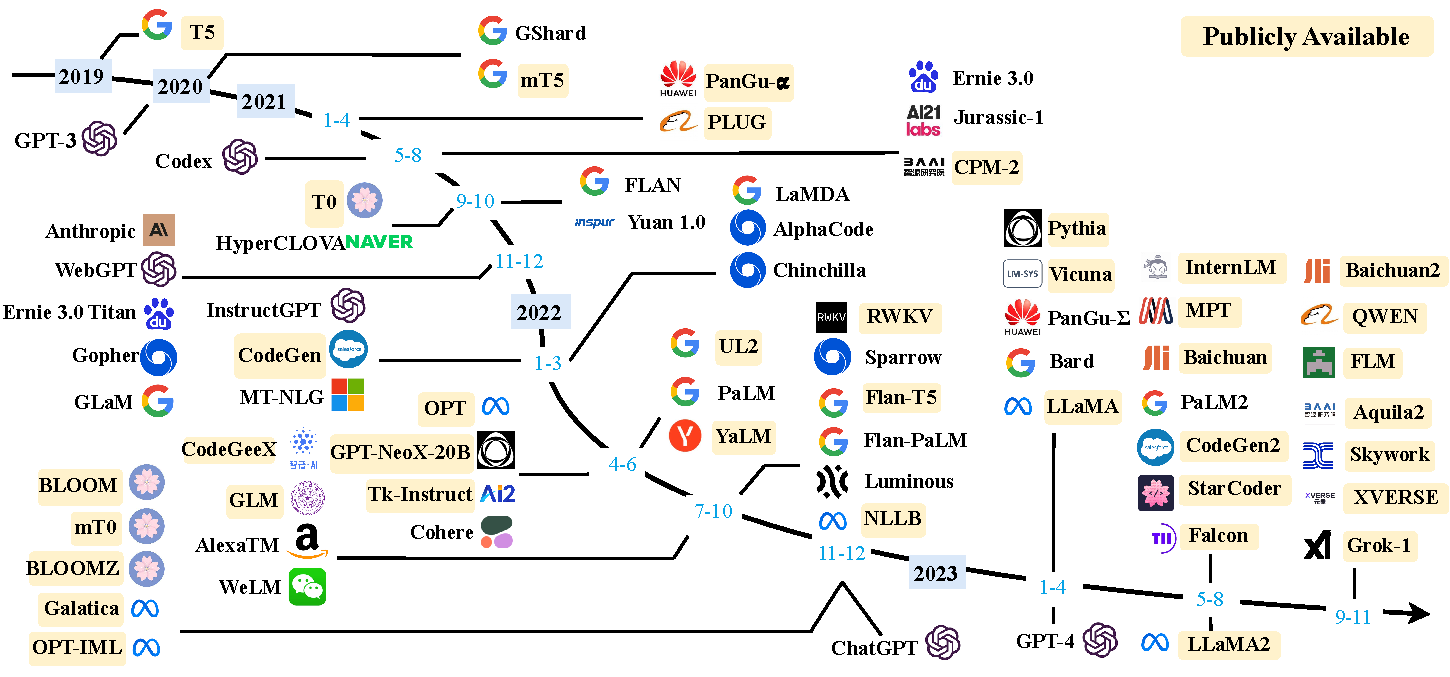
\includegraphics[width=\textwidth]{images/LLMs-1124-final.pdf}
    \caption{A timeline of existing large language models (having a size larger than 10B) in recent years. The timeline was established mainly according to the release date (\eg the submission date to arXiv) of the technical paper for a model. If there was not a corresponding paper, we set the date of a model as the earliest time of its public release or announcement. We mark the LLMs with publicly available model checkpoints in yellow color. Due to the space limit of the figure, we only include the LLMs with publicly reported evaluation results. }
    \label{fig:llms_timeline}
\end{figure*}


\begin{table*}[htbp]
\centering
\caption{Statistics  of  large language models (having a size larger than 10B in this survey) in recent years, including the capacity evaluation, pre-training data scale (either in the number of tokens or storage size)  and hardware resource costs. In this table, we only include LLMs with a public paper about the technical details.
Here, ``Release Time"   indicates the date when the corresponding paper was officially released. ``Publicly Available" means  that the model checkpoints can be publicly accessible while ``Closed Source"  means the opposite.
``Adaptation'' indicates whether the model has been with subsequent fine-tuning: IT denotes instruction tuning and RLHF denotes reinforcement learning with human feedback.
``Evaluation'' indicates whether the model has been evaluated with  corresponding abilities in their original paper: ICL denotes in-context learning and CoT denotes chain-of-thought. ``*'' denotes the largest publicly available version. 
}
\label{tab:resource_model}
\footnotesize
\renewcommand\tabcolsep{2.5pt}
\begin{tabular}{llcrccccccccc}
\toprule
  &  &   & \multicolumn{1}{c}{}  & & \multicolumn{2}{c}{\textbf{Adaptation}} &   &    & &    & \multicolumn{2}{c}{\textbf{Evaluation}}   \\
\multirow{-2}{*}{}    & \multirow{-2}{*}{\textbf{Model}} & \multirow{-2}{*}{\textbf{\begin{tabular}[c]{@{}c@{}}Release\\ Time\end{tabular}}} & \multicolumn{1}{c}{\multirow{-2}{*}{\textbf{\begin{tabular}[c]{@{}c@{}}Size\\ (B)\end{tabular}}}} & \multirow{-2}{*}{\textbf{\begin{tabular}[c]{@{}c@{}}Base\\ Model\end{tabular}}} & \textbf{IT}   & \textbf{RLHF} & \multirow{-2}{*}{\textbf{\begin{tabular}[c]{@{}c@{}}Pre-train\\ Data Scale\end{tabular}}} & \multirow{-2}{*}{\textbf{\begin{tabular}[c]{@{}c@{}}Latest Data\\ Timestamp\end{tabular}}} & \multirow{-2}{*}{\textbf{\begin{tabular}[c]{@{}c@{}}Hardware\\ (GPUs / TPUs)\end{tabular}}} & \multirow{-2}{*}{\textbf{\begin{tabular}[c]{@{}c@{}}Training\\ Time\end{tabular}}} & \textbf{ICL} & \textbf{CoT} \\
\midrule
  & T5~\cite{Raffel-JMLR-2020-Exploring}   & Oct-2019    & 11    & -   & - & - & {1T tokens}    & Apr-2019 & 1024 TPU v3 & -  & $\checkmark$ & -    \\
  & mT5~\cite{Xue-NAACL-2021-mT5}  & Oct-2020    & 13    & -   & - & - & 1T tokens & - & -   & -  & $\checkmark$ & - \\
  &  {PanGu-$\alpha$}~\cite{Zeng-arxiv-2021-PanGualpha}   & Apr-2021    & 13*    & -  &  - & - & 1.1TB   & -  & 2048 Ascend 910 &  -  & $\checkmark$ & - \\
  & CPM-2~\cite{Zhang-arXiv-2021-CPM-2}    & Jun-2021    & 198   & -   & - & - & {2.6TB}  & -  & - & - & -       & -    \\
  & T0~\cite{Sanh-ICLR-2022-Multitask}   & Oct-2021    & 11    & T5  & $\checkmark$  & - & -   & -  & 512 TPU v3  & 27 h   & $\checkmark$ & - \\
  & CodeGen~\cite{nijkamp-arxiv-2022-Codegen}  & Mar-2022    & 16    & -   & - & - & 577B tokens & -  & -   & -  & $\checkmark$ & -  \\
  & GPT-NeoX-20B~\cite{Black-CoRR-2022-GPT} & Apr-2022    & 20    & -   & - & - & 825GB & - & 96 40G A100 & -  & $\checkmark$ & -      \\
  & Tk-Instruct~\cite{Wang-EMNLP-2022-Super}  & Apr-2022    & 11    & T5  & $\checkmark$  & - & - & -  & 256 TPU v3   & 4 h  & $\checkmark$    & -    \\
  & UL2~\cite{Tay-arxiv-2022-UL2}  & May-2022    & 20    & -   & - & - & 1T tokens & Apr-2019 & 512 TPU v4  & -  & $\checkmark$ & $\checkmark$    \\
  & OPT~\cite{Zhang-arxiv-2022-OPT}  & May-2022    & 175   & -   & - & - & 180B tokens   & -  & 992 80G A100    & -  & $\checkmark$  & -    \\
  & NLLB~\cite{Marta-arxiv-2022-NLLB}  & Jul-2022    & 54.5   & -   & - & - & -  & -  & -   & -  & $\checkmark$  & -    \\
  & CodeGeeX~\cite{Zheng-arXiv-2023-CodeGeex}    & Sep-2022    & 13    & -   & - & - & 850B tokens   & - & 1536 Ascend 910 & 60 d   & $\checkmark$ & - \\
  & GLM~\cite{Zeng-arxiv-2022-GLM}  & Oct-2022    & 130   & -   & - & - & 400B tokens   & -  & 768 40G A100    & 60 d  & $\checkmark$ & -    \\
  & Flan-T5~\cite{Chung-arxiv-2022-Scaling}  & Oct-2022    & 11    & T5  & $\checkmark$  & - & - & -  & -   & -  & $\checkmark$ & $\checkmark$  \\
  & BLOOM~\cite{Scao-arxiv-2022-BLOOM}    & Nov-2022    & 176   & -   & - & - & 366B tokens & -  & 384 80G A100    & 105 d  &  $\checkmark$    & -    \\
  & mT0~\cite{Muennighoff-2022-arxiv-Crosslingual}  & Nov-2022    & 13    & mT5 & $\checkmark$  & - & - & -  & -   & -  & $\checkmark$ & - \\
  & Galactica~\cite{Taylor-arxiv-2022-Galactica} & Nov-2022    & 120   & -   & - & - & 106B tokens & -  & -   & -  & $\checkmark$ & $\checkmark$    \\
  & BLOOMZ~\cite{Muennighoff-2022-arxiv-Crosslingual}   & Nov-2022    & 176   & BLOOM   & $\checkmark$  & - & - & -  & -   & -  & $\checkmark$ & - \\
  & OPT-IML~\cite{Iyer-arxiv-2022-OPT}  & Dec-2022    & 175   & OPT & $\checkmark$  & - & - & -  & 128 40G A100   & -  & $\checkmark$ & $\checkmark$    \\
  & LLaMA~\cite{Touvron-arxiv-2023-LLaMA}    & Feb-2023    & 65    & -   & - & - & 1.4T tokens   & - & 2048 80G A100 & 21 d   & $\checkmark$ & -    \\
  & Pythia~\cite{Biderman-arxiv-2023-Pythia}    & Apr-2023    & 12    & -   & - & - & 300B tokens   & - & 256 40G A100 & -  & $\checkmark$ & - \\
  & CodeGen2~\cite{Nijkamp-2023-codegen2-arxiv}    & May-2023    & 16    & -   & - & - & 400B tokens   & - & - & -  & $\checkmark$ & - \\
  & StarCoder~\cite{Li-2023-arxiv-Starcoder}    & May-2023    & 15.5    & -   & - & - & 1T tokens   & - & 512 40G A100 & -  & $\checkmark$ & $\checkmark$ \\
   & LLaMA2~\cite{Touvron-2023-llama2-arxiv}  & Jul-2023    & 70   & - & $\checkmark$   & $\checkmark$ & 2T tokens & -  & 2000 80G A100   & -  & $\checkmark$ & - \\
    & Baichuan2~\cite{yang-2023-baichuan2}  & Sep-2023    & 13   & - & $\checkmark$   & $\checkmark$ & 2.6T tokens & -  & 1024 A800   & -  & $\checkmark$ & - \\
    & QWEN~\cite{bai-2023-qwen}  & Sep-2023    & 14   & - & $\checkmark$   & $\checkmark$ & 3T tokens & -  & -   & -  & $\checkmark$ & - \\
    & FLM~\cite{Li-arxiv-2023-FLM}  & Sep-2023    & 101   & - & $\checkmark$  & - & 311B tokens & -  & 192 A800   & 22 d  & $\checkmark$ & - \\
\multirow{-18}{*}{\begin{tabular}[c]{@{}c@{}}Publicly\\ Available\end{tabular}}  & Skywork~\cite{wei-2023-skywork}  & Oct-2023    & 13   & - & -    & - & 3.2T tokens & -  & 512 80G A800   & -  & $\checkmark$ & - \\

\midrule
\midrule
  & GPT-3~\cite{Brown-NeurIPS-2020-Language}    & May-2020    & 175   & -   & - & - & {300B tokens} & -  & -   & -  & $\checkmark$ & -       \\
  & GShard~\cite{Lepikhin-ILR-2021-GShard}   & Jun-2020    & 600   & -   & - & - & 1T tokens & -  & 2048 TPU v3 & 4 d & -    & -       \\
  & Codex~\cite{Chen-arxiv-2021-evaluating}    & Jul-2021    & 12    & GPT-3   & - & - & 100B tokens & May-2020 & -   & -  & $\checkmark$    & - \\
  & ERNIE 3.0~\cite{Sun-arXiv-2021-ERNIE3.0}    & Jul-2021    & 10    & -   & - & - & 375B tokens & - & 384 V100   & -  & $\checkmark$ & -    \\
  & Jurassic-1~\cite{lieber-2021-jurassic}   & Aug-2021    & 178   & -   & - & - & 300B tokens   & -  & 800 GPU & -  & $\checkmark$    & -       \\
  & HyperCLOVA~\cite{Kim-EMNLP-2021-HyperCLOVA}   & Sep-2021    & 82    & - & -  & - &  300B tokens  & - & 1024 A100   & 13.4 d  & $\checkmark$ & -      \\
  & FLAN~\cite{Wei-ICLR-2022-Finetuned} & Sep-2021    & 137   & LaMDA-PT   & $\checkmark$  & - & -  & -  & 128 TPU v3  & 60 h   & $\checkmark$  & -    \\
  & Yuan 1.0~\cite{Wu-arxiv-2021-Yuan}   & Oct-2021    & 245    &  - & -  & - &  180B tokens  &  -  & 2128 GPU  &  -  & $\checkmark$ & - \\
  & Anthropic~\cite{Askell-arxiv-2021-Anthropic}   & Dec-2021    & 52   & -   & - & - & {400B tokens}   & - & -   & -  & $\checkmark$    & -        \\
  & WebGPT~\cite{Nakano-arxiv-2021-WebGPT}   & Dec-2021    & 175   & GPT-3   & - & $\checkmark$  & - & -  & -   & -  & $\checkmark$ &  -    \\
  & Gopher~\cite{Rae-arxiv-2021-Scaling}   & Dec-2021    & 280   & -   & - & - & 300B tokens   & -  & 4096 TPU v3 & 920 h  & $\checkmark$    & -        \\
  & ERNIE 3.0 Titan~\cite{Wang-arxiv-2021-ERNIE}   & Dec-2021    & 260    &  - & -  & - &  -  & - & -  & -  & $\checkmark$ & -  \\
  & GLaM~\cite{Du-ICML-2022-GLaM} & Dec-2021    & 1200  & -   & - & - & 280B tokens   & -  & 1024 TPU v4 & 574 h  & $\checkmark$ & -       \\
  & LaMDA~\cite{Thoppilan-CoRR-2022-LaMDA}    & Jan-2022    & 137   & -   & - & - & 768B tokens  & -  & 1024 TPU v3 & 57.7 d & -    & -       \\
  & MT-NLG~\cite{Smith-CoRR-2022-Using}   & Jan-2022    & 530   & -   & - & - & {270B tokens}   & - & 4480 80G A100   & -  & $\checkmark$    & -        \\
  & AlphaCode~\cite{Li-Science-2022-AlphaCode}    & Feb-2022    & 41    & -   & - & - & 967B tokens & Jul-2021 & -   & -  & -    & -        \\
  & InstructGPT~\cite{Ouyang-arxiv-2022-Training}  & Mar-2022    & 175   & GPT-3   & $\checkmark$  & $\checkmark$  & -  & -  & -   & -  & $\checkmark$  & -    \\
  & Chinchilla~\cite{Hoffmann-arxiv-2022-Training}   & Mar-2022    & 70    & -   & - & - & 1.4T tokens   & -  & -   & -  & $\checkmark$    & -        \\
  & PaLM~\cite{Chowdhery-arxiv-2022-PaLM} & Apr-2022    & 540   & -   & - & - & 780B tokens   & -  & 6144 TPU v4 & -  & $\checkmark$       & $\checkmark$ \\
  & AlexaTM~\cite{Soltan-arxiv-2022-AlexaTM20B}  & Aug-2022    & 20    & -   & - & - & 1.3T tokens   & -  & 128 A100    & 120 d  & $\checkmark$ & $\checkmark$       \\
  & Sparrow~\cite{Glaese-arxiv-2022-Improving}  & Sep-2022    & 70    & -   & - & $\checkmark$  & - & -  & 64 TPU v3   & -  & $\checkmark$    & -       \\
  & WeLM~\cite{Su-arxiv-2022-WeLM}  & Sep-2022    & 10    & -   & - & -  & 300B tokens & -  & 128 A100 40G   & 24 d  & $\checkmark$    & -       \\
  & U-PaLM~\cite{Tay-arxiv-2022-Transcending}   & Oct-2022    & 540   & PaLM & - & - & - & -  & 512 TPU v4  & 5 d    & $\checkmark$       & $\checkmark$ \\
  & Flan-PaLM~\cite{Chung-arxiv-2022-Scaling}    & Oct-2022    & 540   & PaLM    & $\checkmark$  & - & - & -  & 512 TPU v4  & 37 h   & $\checkmark$ & $\checkmark$  \\
  & Flan-U-PaLM~\cite{Chung-arxiv-2022-Scaling}  & Oct-2022    & 540   & U-PaLM  & $\checkmark$  & - & - & -  & -   & -  & $\checkmark$ & $\checkmark$  \\
  & GPT-4~\cite{OpenAI-OpenAI-2023-GPT-4}    & Mar-2023    & - & -   & $\checkmark$  & $\checkmark$  & - & -  & -   & -  & $\checkmark$ & $\checkmark$  \\
  & {PanGu-$\Sigma$}~\cite{Ren-arXiv-2023-PanGusigma}  & Mar-2023  & 1085 & {PanGu-$\alpha$}   & -  & -  & 329B tokens & -  & 512 Ascend 910   & 100 d  & $\checkmark$  & -   \\
\multirow{-25}{*}{\begin{tabular}[c]{@{}c@{}}Closed\\ Source\end{tabular}} & PaLM2~\cite{Anil-arxiv-2023-palm2}    & May-2023    & 16 & -   & $\checkmark$  & -  & 100B tokens & -  & -   & -  & $\checkmark$ & $\checkmark$  \\
\bottomrule
\end{tabular}
\end{table*}



\begin{figure*}[h]
    \centering
    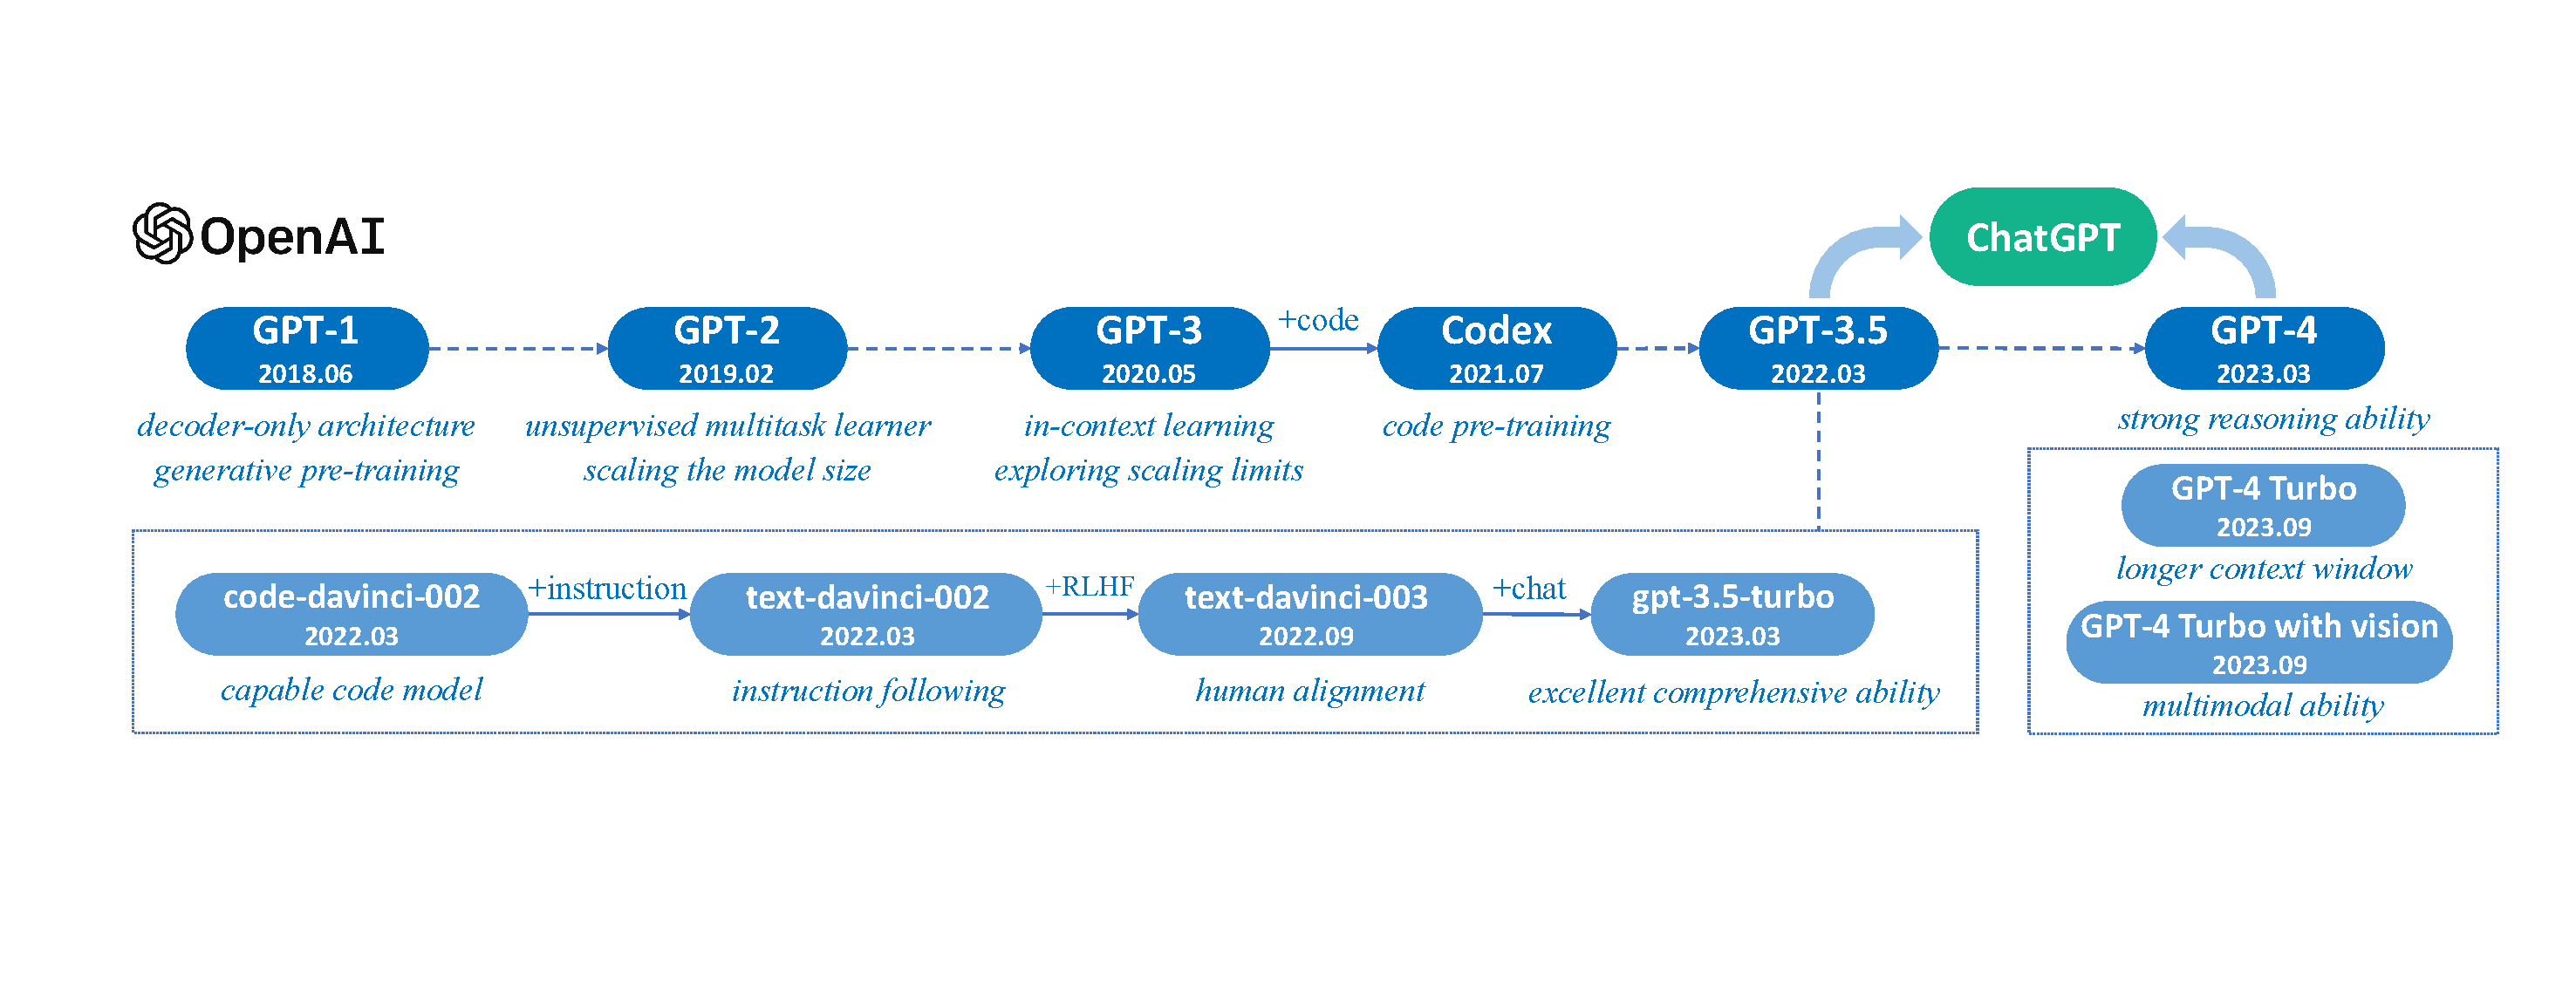
\includegraphics[width=\textwidth]{images/openai-v2.pdf}
    \caption{A brief  illustration for the technical evolution of GPT-series models. We plot this figure mainly based on the papers, blog articles and official APIs from OpenAI. Here,  \emph{solid lines}  denote that there exists an explicit evidence (\eg the official statement that a new model is developed based on a base model) on the evolution path between two models, while \emph{dashed lines} denote a relatively weaker evolution relation. }
    \label{fig:openai}
\end{figure*}


\subsection{Technical Evolution  of GPT-series Models}\label{sec-GPT-series}

Due to the  excellent capacity in communicating  with humans,  ChatGPT has ignited the excitement of the AI community since its release.   
ChatGPT is developed based on the powerful GPT model with specially optimized conversation  capacities.   
Considering the ever-growing interest in ChatGPT and GPT models, we add a special discussion about the technical evolution of the GPT-series models, to briefly summarize the progress how they have been developed in the past years. %
{Meanwhile, we drew a schematic diagram depicting the technological evolution of the GPT-series models in Figure~\ref{fig:openai}.} 
The basic principle underlying GPT models is to compress the world knowledge into the decoder-only Transformer model by language modeling,  such that it can  recover (or memorize) the semantics of world knowledge and serve as a general-purpose task solver. Two key points to the success are  (I)   training decoder-only Transformer language models that can \emph{accurately predict the next word}  and (II) \emph{scaling  up the size of  language models}.   
Overall, the research of OpenAI on LLMs can be roughly divided into the following stages\footnote{Note that the discussion of this part can be somewhat subjective. The overall viewpoints and summaries are made based on the understanding of the survey authors by reading  the papers, blog articles, interview reports and APIs released by OpenAI.  }.  

\paratitle{Early Explorations}. According to one interview with Ilya Sutskever\footnote{\url{https://hackernoon.com/an-interview-with-ilya-sutskever-co-founder-of-openai}} (a co-founder and chief scientist of OpenAI), the idea of approaching   intelligent systems  with language models was already explored in the early days of OpenAI, while it was attempted with recurrent neural networks~(RNN)~\cite{Radford-CoRR-2017-Learning}. With the advent of Transformer, OpenAI developed two initial GPT models, namely GPT-1~\cite{radford-openai-2018-improving} and GPT-2~\cite{radford-blog-2019-language}, which can be considered as the foundation to  more powerful models subsequently \ie GPT-3 and GPT-4.   

$\bullet$ \emph{GPT-1}. In 2017, the Transformer model~\cite{Vaswani-NIPS-2017-Attention} was introduced by Google, and the OpenAI team quickly adapted their language modeling work to this new neural network architecture. They released the first GPT model in 2018, \ie GPT-1~\cite{radford-openai-2018-improving}, and coined the abbreviation term \emph{GPT} as the model name,  standing for \emph{Generative Pre-Training}. GPT-1 was developed based on a generative, decoder-only Transformer architecture, and adopted a hybrid  approach of  unsupervised pretraining and supervised fine-tuning. 
GPT-1 has set up the core architecture for the GPT-series models and established the underlying principle to model natural language text, \ie predicting the next word.  

$\bullet$ \emph{GPT-2}. Following a similar architecture of GPT-1,  GPT-2~\cite{radford-blog-2019-language} increased the parameter scale to 1.5B, which was trained with a large webpage dataset WebText. As claimed in the paper of GPT-2, it sought to perform tasks via unsupervised language modeling, without  explicit fine-tuning using labeled data. To motivate the approach, they  introduced a   probabilistic form for  multi-task solving, \ie  $p(output|input, task)$ (similar approaches have been adopted in \cite{McCann-CoRR-2018-The}), which predicts the output conditioned on the input and task information.  To model this conditional probability,  language text can be naturally employed as a unified way to  format  input, output and task information.  In this way, the process of solving a task  can be cast as a word prediction problem for generating the solution text. Further, they introduced  a more formal claim for this idea: ``Since the (task-specific) supervised objective is the same as the unsupervised (language modeling) objective but only evaluated on a subset of the sequence, the global minimum of the unsupervised objective is also the global minimum of the supervised objective (for various tasks)''~\cite{radford-blog-2019-language}\footnote{To better understand this sentence, we put some explanation words in parentheses.}. 
A basic understanding of this claim is that each (NLP) task can be considered as the word prediction problem based on a subset of the world text. Thus,  unsupervised language modeling could be capable in solving various tasks, if it was trained to have sufficient capacity in recovering the world text.   
These early discussion in GPT-2's paper echoed in the interview of Ilya Sutskever by Jensen Huang: ``What the neural network learns is some representation of the process that produced the text. This text is actually a projection of the world...the more accurate you are in predicting the next word, the higher the fidelity, the more resolution you get in this process...''\footnote{\url{https://lifearchitect.ai/ilya/}}.   
 

\paratitle{Capacity Leap}. Although GPT-2 is intended to be an  ``unsupervised multitask learner'', it overall has an inferior performance compared with supervised fine-tuning state-of-the-art methods.  
Because it has a relatively small model size, it has been widely fine-tuned in downstream tasks, especially the dialog tasks~\cite{Zhang-ACL-2020-DIALOGPT,Ham-ACL-2020-End}. Based on GPT-2, GPT-3 demonstrates a  key capacity leap by scaling of the (nearly same) generative pre-training architecture.  
 
$\bullet$ \emph{GPT-3}. GPT-3~\cite{Brown-NeurIPS-2020-Language} was released in 2020, which scaled the model parameters to an ever larger size of 175B. In the GPT-3's paper, it formally introduced the concept of in-context learning~(ICL)\footnote{GPT-2 essentially used ICL for unsupervised task learning, though it wasn't called ICL at that time.  }, which utilizes LLMs in a few-shot or zero-shot way. ICL can  teach (or instruct) LLMs to understand the tasks  in the form of natural language text. 
With ICL, the pre-training and utilization of LLMs converge to the same language modeling paradigm: pre-training predicts the following text sequence conditioned on the context, while ICL predicts the correct task solution, which can be  also formatted as a text sequence, given the task description and demonstrations. 
GPT-3 not only demonstrates very excellent performance in a variety of NLP tasks, but also on a number of specially designed tasks that require the abilities of reasoning or domain adaptation. Although the GPT-3's paper does not explicitly discuss the emergent abilities of LLMs, we can observe  large performance leap that might transcend the basic scaling law~\cite{Kaplan-arxiv-2020-Scaling}, \eg  larger models have significantly stronger ICL ability (illustrated in the original Figure~1.2 of the GPT-3's  paper~\cite{Brown-NeurIPS-2020-Language}).  Overall, GPT-3 can be viewed as a remarkable landmark in the journey evolving  from PLMs to LLMs.  It has empirically proved that scaling the neural networks to a  significant size can lead to a huge increase in model capacity. 


\paratitle{Capacity Enhancement}. Due to the strong capacities,  GPT-3  has been the base model to develop even more capable LLMs for OpenAI. Overall, OpenAI has explored  two major approaches to further improving the GPT-3 model, \ie training on code data and alignment with human preference, which are detailed as follows. 

$\bullet$ \emph{Training on code data}. A major limitation of the original  GPT-3 model  (pre-trained on plain text) lies in the lack of the reasoning ability on complex tasks, \eg completing the code and solving math problems. To enhance this ability,  Codex~\cite{Chen-arxiv-2021-evaluating} was introduced by OpenAI in July 2021, which was a GPT model fine-tuned on 
a large corpus of GitHub code. It demonstrated that Codex can solve very difficult programming problems, and also lead to a significant performance  improvement in solving math problems~\cite{Drori-CoRR-2021-A}. Further, a contrastive approach~\cite{Neelakantan-CoRR-2022-Text} to training text and code embedding was reported in January 2022, which was shown to improve a series of related tasks (\ie  linear-probe classification, text search and code search). Actually, the GPT-3.5 models are developed based on a code-based GPT model (\ie \texttt{code-davinci-002}), which indicates that training on code data is a very useful practice to improve the model capacity  of GPT models, especially the reasoning ability.  
Furthermore, there is  also a speculation  that training on code data can greatly increase the chain-of-thought prompting abilities of LLMs~\cite{FU-blog-2022-how}, while it is still worth further investigation with more thorough verification. 


$\bullet$ \emph{Human alignment}. The related research of human alignment can be dated back to the year 2017 (or earlier) for OpenAI: a blog article entitled ``learning from human preferences''\footnote{\url{https://openai.com/research/learning-from-human-preferences}} was posted on the OpenAI blog describing a work that applied   reinforcement learning~(RL) to learn from the \emph{preference comparisons}  annotated by  humans~\cite{Christiano-NeurIPS-2017-Deep} (similar to the \emph{reward training}  step in the aligning algorithm of InstructGPT in Figure~\ref{fig:RLHF}). 
Shortly after the release of this RL paper~\cite{Christiano-NeurIPS-2017-Deep}, the paper of the Proximal Policy Optimization~(PPO)~\cite{schulman-arxiv-2017-proximal} was published in July 2017, which now has been the foundational RL algorithm for learning from human preferences~\cite{Ouyang-arxiv-2022-Training}. 
Later in January 2020, GPT-2 was fine-tuned using the aforementioned RL algorithms~\cite{Christiano-NeurIPS-2017-Deep,schulman-arxiv-2017-proximal}, which leveraged human preferences to improve the capacities of GPT-2 on NLP tasks. In the same year, another work~\cite{Stiennon-arxiv-2020-learning} trained a summarization  model for optimizing  human preferences in a similar way. 
Based on these prior work, InstructGPT~\cite{Ouyang-arxiv-2022-Training} was proposed in January 2022 to improve the GPT-3 model for human alignment, which formally established a three-stage    \emph{reinforcement learning from human feedback~(RLHF)} algorithm. 
Note that it seems that the wording of ``\emph{instruction tuning}'' has seldom been used in OpenAI's paper and documentation, which is substituted by \emph{supervised fine-tuning on human demonstrations} (\ie the first step of the RLHF algorithm~\cite{Ouyang-arxiv-2022-Training}). 
In addition to improving the instruction following capacity, the RLHF algorithm is particularly useful to mitigate the issues of generating harm or toxic content for LLMs, which is key to the safe deployment of LLMs in practice. 
 OpenAI describes  their approach to alignment research in a technical article~\cite{OpenAI-blog-2022-alignment},  which has summarized three promising directions: ``training AI systems to use human feedback, to  assist human evaluation and to do  alignment research''.  

These enhancement techniques lead to the improved GPT-3 models with stronger capacities, which are called GPT-3.5 models  by OpenAI (see the discussion about the OpenAI API in Section~\ref{subsec-models-apis}).

%

\paratitle{The Milestones of Language Models}. 
Based on all the exploration efforts, two major milestones have been achieved by OpenAI, namely  ChatGPT~\cite{OpenAI-blog-2022-ChatGPT} and GPT-4~\cite{OpenAI-OpenAI-2023-GPT-4}, which have largely raised the capacity bar of existing AI systems. 

$\bullet$ \emph{ChatGPT}. In November 2022, OpenAI released the conversation model  ChatGPT, based on the GPT models (GPT-3.5 and GPT-4). As the official blog article introduced~\cite{OpenAI-blog-2022-ChatGPT}, ChatGPT was trained in a similar way as InstructGPT (called ``a sibling model to InstructGPT'' in the original post), while specially optimized for dialogue. 
They reported a difference between the training of ChatGPT and InstructGPT in  the data collection setup: human-generated conversations (playing both the roles of user and AI) are combined with the InstructGPT dataset in a dialogue format for training ChatGPT.  
ChatGPT exhibited superior capacities in communicating with humans: possessing  a vast store of knowledge,  skill at reasoning on mathematical problems, tracing the context accurately in multi-turn dialogues, and aligning well with human values for safe use. Later on, the plugin mechanism has been supported in ChatGPT, which further  extends the capacities of ChatGPT with existing tools or apps.
So far, it seems to be the ever most powerful chatbot in the AI history. The launch of ChatGPT has a significant impact on the AI research in the future, which sheds light on the exploration of  human-like AI systems. 

$\bullet$ \emph{GPT-4}. As another remarkable progress,  GPT-4~\cite{OpenAI-OpenAI-2023-GPT-4} was released in March 2023, which extended the text input to multimodal signals. 
Overall, GPT-4 has  stronger capacities  in solving complex tasks than GPT-3.5, showing a large performance improvement on many evaluation tasks. 
A recent study~\cite{Bubeck-arxiv-2023-Sparks}  investigated the capacities of GPT-4 by conducting qualitative tests with human-generated  problems, spanning a diverse range of difficult  tasks, and showed  that GPT-4 can achieve more superior performance than prior GPT models such as ChatGPT. 
Furthermore, GPT-4  responds more safely to  malicious or provocative queries, due to a six-month iterative alignment (with an additional  safety reward signal in the RLHF training). 
In the technical report, OpenAI has emphasized how to safely develop GPT-4 and applied  a number of  intervention strategies  to mitigate the possible issues of LLMs, such as hallucinations, privacy and overreliance. For example, they introduced the mechanism called \emph{red teaming}~\cite{Ganguli-arxiv-2022-Red}  to reduce the harm or toxic content generation. 
As another important aspect, GPT-4 has been developed on a well-established deep learning infrastructure with improved optimization methods. They  introduced a new mechanism called \emph{predictable scaling} that can  accurately predict the final performance with a small proportion of compute during model training. 

{
$\bullet$ \emph{GPT-4V, GPT-4 turbo, and beyond}. Based on the work done for GPT-4~\cite{OpenAI-OpenAI-2023-GPT-4}, OpenAI further released GPT-4V in September 2023, 
which focused on the safe deployment of the vision capabilities of GPT-4. In the GPT-4V's  system card~\cite{OpenAI-OpenAI-2023-GPT-4v}, it has extensively discussed the  assessment and mitigation of risks related to visually augmented inputs.
Specially, GPT-4V  exhibited strong vision capacities in various application scenarios, showing the great potential as a powerful multimodal learning  system. 
More recently, in November 2023, OpenAI 
 released an upgraded generation of GPT-4 model at DevDay, named \emph{GPT-4 Turbo}, with a series of  technical improvements. 
 GPT-4 Turbo is featured by the improved model capacity (more capable than GPT-4), the extended knowledge source (up to April 2023), long context window (up to 128k tokens), optimized model performance (cheaper price), and other useful functionality updates (function call, reproducible outputs, etc.). 
 At the same time,  Assistants API was  launched to ease the rapid development of  agent-like assistants. With this API, developers can easily create goal-oriented assistants within their applications, by leveraging specific instruction,  extra knowledge and tool use. Furthermore, multimodal capacities (see, hear, and speak) were also enhanced in this new release, supported by  GPT-4 Turbo with vision, DALL·E 3, Text-to-speech~(TTS), and Listen to voice samples. 
 These improvements  have greatly extended the capacity scope and enhanced the task  performance of GPT models. %
 More importantly, the application ecosystem will be greatly strengthened with the technology upgrade in improved models, APIs, and functionalities.  
 }
 





Despite the huge progress, there are still limitations with these superior LLMs, \eg generating hallucinations with factual errors or potentially risky response within some specific context~\cite{OpenAI-OpenAI-2023-GPT-4}. More limitations or issues of LLMs will be discussed in Section~\ref{sec-evaluation}. 
It poses  long-standing research challenges to develop more capable, safer LLMs. 
From the perspective of engineering, OpenAI has adopted an iterative deployment strategy~\cite{OpenAI-blog-2022-lessons}  to develop the models and products by following a five-stage development and deployment life-cycle, which aims to effectively reduce the potential risks of using the models. 
In the following, we will dive into the technical details in order to have a specific understanding of how they have been  developed. 




\begin{figure*}
    \centering
    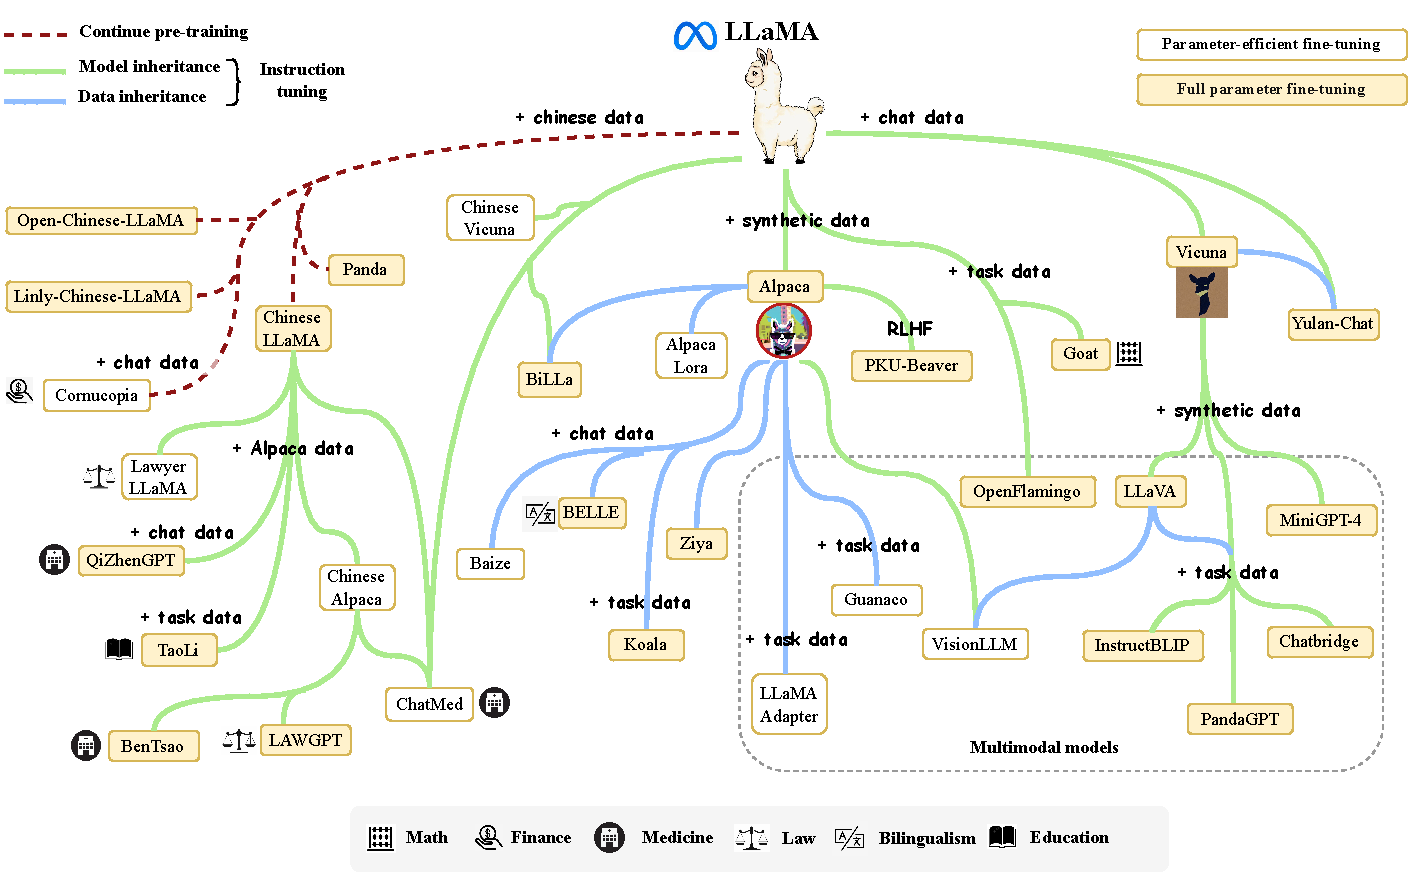
\includegraphics[width=\textwidth]{images/llama-0628-final.pdf}
    \caption{An evolutionary graph of the research  work conducted on LLaMA. Due to the huge number, we cannot include  all the LLaMA variants in this figure, even much excellent work. To support incremental update, we share the source file of this figure, and welcome the readers to include the desired models by submitting the pull requests on our GitHub page. }
    \label{fig:llama_family}
    
\end{figure*}

 

\section{Resources of LLMs}
\label{sec-resource}
It is by no means an easy job  to develop or reproduce LLMs, considering the challenging technical issues and huge demands of computation resources.  
A feasible way is to learn experiences from existing LLMs and reuse publicly available resources for incremental development or experimental study.  In this section, we briefly summarize the publicly available resources for developing LLMs, including model checkpoints (or APIs), corpora and libraries.



\subsection{Publicly Available Model Checkpoints or APIs}\label{subsec-models-apis}
Given the huge cost of model pre-training, well-trained model checkpoints are critical to the study and development  of LLMs  for the research community. Since the parameter scale is a key factor to consider for using LLMs, we categorize these public models into two scale levels (\ie \emph{tens of billions of parameters} and  \emph{hundreds of billions of parameters}), 
which is useful for  users to identify the suitable resources according to their resource budget.    In addition, for inference, we can directly employ public APIs to perform  our tasks, without running the model 
{locally}.  Next, we introduce the publicly available model checkpoints and APIs. 


\paratitle{Models with Tens of Billions of Parameters}. 
{Most of the models in  this category have a parameter scale ranging from 10B to 20B, {except LLaMA~\cite{Touvron-arxiv-2023-LLaMA} and LLaMA2~\cite{Touvron-2023-llama2-arxiv} (containing 70B parameters in the largest version)}, NLLB~\cite{Marta-arxiv-2022-NLLB} (containing 54.5B parameters in the largest version), and Falcon~\cite{Falcon40b} (containing 40B parameters in the largest version).  }
Other  models within this range include mT5~\cite{Xue-NAACL-2021-mT5}, PanGu-$\alpha$~\cite{Zeng-arxiv-2021-PanGualpha}, T0~\cite{Sanh-ICLR-2022-Multitask}, GPT-NeoX-20B~\cite{Black-CoRR-2022-GPT}, CodeGen~\cite{nijkamp-arxiv-2022-Codegen}, UL2~\cite{Tay-arxiv-2022-UL2}, Flan-T5~\cite{Chung-arxiv-2022-Scaling}, and mT0~\cite{Muennighoff-2022-arxiv-Crosslingual}.
Among them, Flan-T5~(11B version) can serve as a premier model for research on instruction tuning, since it explores the instruction tuning from three aspects~\cite{Chung-arxiv-2022-Scaling}: increasing the number of tasks, scaling the model size, and fine-tuning with chain-of-thought prompting data. 
Besides, CodeGen~(11B version), as an autoregressive language model designed for generating code, {can be considered as a good candidate for exploring the code generation ability.}
It also introduces a new benchmark MTPB~\cite{nijkamp-arxiv-2022-Codegen} specially for multi-turn program synthesis, which is composed by 115 expert-generated problems. To solve these problems, it requires LLMs to acquire sufficient programming knowledge (\eg math, array operations, and algorithms).  %
{More recently, CodeGen2~\cite{Nijkamp-2023-codegen2-arxiv} has been released to explore the impact of choices in model architecture, learning algorithms, and data distributions on the model. As another LLM specialized in coding abilities, StarCoder~\cite{Li-2023-arxiv-Starcoder} has also achieved excellent results. 
As for multilingual tasks, mT0~(13B version) might be a good candidate model, which has been fine-tuned on multilingual tasks with multilingual prompts. 
{Furthermore, PanGu-$\alpha$~\cite{Zeng-arxiv-2021-PanGualpha} shows good performance in Chinese downstream tasks in zero-shot or few-shot settings, which is developed  based on the deep learning framework MindSpore~\cite{Huawei-Springer-2022-MindSpore}. 
Note that PanGu-$\alpha$~\cite{Zeng-arxiv-2021-PanGualpha} holds multiple versions of models (up to 200B parameters), while the largest public version has 13B parameters.  }
As a popular LLM, LLaMA~(65B version)~\cite{Touvron-arxiv-2023-LLaMA}, which contains approximately five times as many parameters as other models, has exhibited superior performance in tasks related to instruction following.  %
{Compared to LLaMA, LLaMA2~\cite{Touvron-2023-llama2-arxiv} has made more explorations in reinforcement learning from human feedback~(RLHF) and developed a chat-oriented version called \emph{LLaMA-chat}, which generally outperforms existing open-source models across a range of helpfulness and safety benchmarks.}
{Due to the openness and effectiveness, 
LLaMA has attracted significant attention from the research community, and many efforts~\cite{alpaca, vicuna2023, ChatLLaMA, ColossalChat} have been devoted to fine-tuning or continually pre-training its different model versions  for implementing new models or tools. }  {More recently, {Falcon~\cite{Falcon40b}}, as another open-source LLM, has also achieved very excellent  performance on open benchmarks. It is featured by a more careful data cleaning process to prepare the pre-training data (with a publicly shared dataset \emph{RefinedWeb~\cite{Penedo-2023-arxiv-Refinedweb}). }
Typically, pre-training  models at this scale  require hundreds or even thousands of GPUs or TPUs. For instance, GPT-NeoX-20B uses 12 supermicro servers, each equipped with 8 NVIDIA A100-SXM4-40GB GPUs, while LLaMA utilizes 2,048 A100-80G GPUs as reported in their original publications. To accurately estimate the computation resources needed, it is suggested to use the metrics measuring the number of involved computations such as \emph{FLOPS} (\ie FLoating point number Operations Per Second)~\cite{Kaplan-arxiv-2020-Scaling}. 


\paratitle{Models with Hundreds of Billions of Parameters}. 
For models in this category, only a handful of models have been publicly released. For example, OPT~\cite{Zhang-arxiv-2022-OPT}, OPT-IML~\cite{Iyer-arxiv-2022-OPT}, BLOOM~\cite{Scao-arxiv-2022-BLOOM}, and BLOOMZ~\cite{Muennighoff-2022-arxiv-Crosslingual} have nearly the same number of parameters as GPT-3~(175B version), while GLM~\cite{Zeng-arxiv-2022-GLM} and Galactica~\cite{Taylor-arxiv-2022-Galactica} have 130B and 120B parameters, respectively. 
{Among them, OPT~(175B version), with the instruction-tuned version OPT-IML, has been specially motivated for open sharing, which aims to enable researchers to carry out reproducible research at scale. } 
For research in cross-lingual generalization, BLOOM~(176B version) and BLOOMZ~(176B version) can be used as base models,  due to the competence in multilingual language modeling tasks. 
As a bilingual LLM, GLM has also provided a popular small-sized Chinese chat model ChatGLM2-6B  
 (a updated version for ChatGLM-6B), which is featured with many improvements in efficiency and capacity (\eg quantization, 32K-length context, fast inference rate).   
Models of this scale typically require thousands of GPUs or TPUs to train. For instance, OPT~(175B version) used 992  A100-80GB GPUs, while GLM~(130B version) used  a cluster of 96 NVIDIA DGX-A100 (8x40G) GPU nodes.

\paratitle{LLaMA Model Family}. The collection of LLaMA models~\cite{Touvron-arxiv-2023-LLaMA}  
were introduced by Meta AI in February, 2023, consisting of four sizes (7B, 13B, 30B and 65B).  
Since released, LLaMA has attracted extensive attention from both research and industry communities. 
LLaMA models have achieved very excellent performance on various open benchmarks, which have become the most popular open language models thus far. 
A large number of researchers have extended LLaMA models by either instruction tuning or continual pretraining. In particular, instruction tuning LLaMA has become a major approach to developing customized or specialized models, due to the relatively low computational costs.  
To effectively adapt LLaMA models in non-English languages, it often needs to extend the original vocabulary (trained mainly  on English corpus) or fine-tune it with instructions or data in the target language. 
Among these extended models,  Stanford Alpaca~\cite{Taori-github-2023-Stanford} is the first open instruct-following model fine-tuned based on LLaMA~(7B). It is trained by 52K instruction-following demonstrations generated via self-instruct~\cite{Wang-arXiv-2022-Self} using \texttt{text-davinci-003}. 
The instruction data, named \emph{Alpaca-52K}, and training code have been extensively adopted  in subsequent work, such as Alpaca-LoRA~\cite{Alpaca-LoRA} (a reproduction of Stanford Alpaca using LoRA~\cite{Hu-ICLR-2022-LoRA}), Koala~\cite{koala_blogpost_2023}, and BELLE~\cite{BELLE}. In addition, Vicuna~\cite{vicuna2023} is another popular LLaMA variant,   trained upon user-shared conversations collected from ShareGPT~\cite{ShareGPT}. 
Due to the excellent  performance and availability of the LLaMA model family, many multimodal models incorporate them as the base language models, to achieve strong language understanding and generation abilities. 
Compared with other variants, Vicuna is more preferred in multimodal language models, which have led to the emergence of a variety of popular models, including  LLaVA~\cite{Liu-arxiv-2023-Visual}, MiniGPT-4~\cite{Zhu-arxiv-2023-MiniGPT-4}, InstructBLIP~\cite{Dai-2023-arxiv-InstructBLIP}, and PandaGPT~\cite{su-2023-arxiv-pandagpt}. %
The release of LLaMA has greatly advanced the research progress of LLMs. %
{To  summarize the research work conducted on  LLaMA, we present a brief evolutionary graph in Figure~\ref{fig:llama_family}. 
}


%


\paratitle{Public API of LLMs}.
\label{sec:apis_for_llms}
{Instead of directly using the model copies, APIs provide a more convenient way for common users to use LLMs, without the need of running the model locally. As a representative interface for using LLMs, the APIs for the GPT-series models~\cite{Brown-NeurIPS-2020-Language, Chen-arxiv-2021-evaluating, Ouyang-arxiv-2022-Training, OpenAI-OpenAI-2023-GPT-4} have been widely used for both academia and industry\footnote{{https://platform.openai.com/docs/api-reference/introduction}}. OpenAI has provided  {seven major interfaces to the models in GPT-3 series: \texttt{ada}, \texttt{babbage}, \texttt{curie}, \texttt{davinci} (the most powerful version in GPT-3 series), \texttt{text-ada-001}, \texttt{text-babbage-001}, and \texttt{text-curie-001}.}  Among them, the first four interfaces can be further fine-tuned on the host server of OpenAI.  
In particular, \texttt{babbage}, \texttt{curie}, and \texttt{davinci} correspond to the GPT-3~(1B), GPT-3~(6.7B), and GPT-3~(175B) models, respectively~\cite{Brown-NeurIPS-2020-Language}. 
In addition, there are also two APIs related to Codex~\cite{Chen-arxiv-2021-evaluating}, called \texttt{code-cushman-001} (a powerful and multilingual version of the Codex~(12B)~\cite{Chen-arxiv-2021-evaluating}) and \texttt{code-davinci-002}.
Further, GPT-3.5 series include one base model \texttt{code-davinci-002} and  three enhanced versions, namely \texttt{text-davinci-002}, \texttt{text-davinci-003}, and \texttt{gpt-3.5-turbo}.
As more powerful alternatives, in this year, OpenAI has released the model interfaces for GPT-4 series, including \texttt{gpt-4}, \texttt{gpt-4-32k}, \texttt{gpt-4-1106-preview}~(\ie GPT-4 Turbo) and \texttt{gpt-4-vision-preview}~(\ie GPT-4 Turbo with vision, a multimodal model). 
{It is worth noting that OpenAI has been  maintaining and upgrading these model interfaces (\texttt{gpt-3.5-turbo}, \texttt{gpt-4}, \texttt{gpt-4-32k}), so the API name will actually point to the latest version. } 
Currently, ChatGPT can be  powered by either GPT-3.5 or GPT-4 models.  Overall, one select the suitable model interface based on the specific application scenarios and response requirements.
The detailed usage can be found on their project websites\footnote{https://platform.openai.com/docs/models/overview}.
 

\begin{table}[htbp]
    \centering
    \caption{Statistics of commonly-used data sources. }
    \label{tab:corpora}
    \footnotesize
    \renewcommand\tabcolsep{2.5pt}
    \begin{tabular}{llcc}
    \toprule
    {\textbf{Corpora}} & {\textbf{Size}} &  {\textbf{Source}} & {\textbf{Latest Update Time}} \\
    \midrule
    BookCorpus~\cite{Zhu-ICCV-2015-Aligning} & 5GB   & Books    & Dec-2015 \\
    Gutenberg~\cite{Gutenberg}   & -    & Books    & Dec-2021 \\ 
    C4~\cite{Raffel-JMLR-2020-Exploring}  & 800GB    & CommonCrawl  & Apr-2019 \\
    CC-Stories-R~\cite{Trinh-CoRR-2018-A}  & 31GB    & CommonCrawl  & Sep-2019 \\
    CC-NEWS~\cite{Liu-CoRR-2019-RoBERTa} & 78GB  & CommonCrawl  & Feb-2019 \\
    REALNEWs~\cite{Zellers-NeurIPS-2019-Defending}    & 120GB & CommonCrawl  & Apr-2019 \\
    OpenWebText~\cite{Gokaslan2019OpenWeb} & 38GB  & Reddit links & Mar-2023 \\
    Pushift.io~\cite{Baumgartner-AAAI-2020-The}  & 2TB    & Reddit links & Mar-2023 \\
    Wikipedia~\cite{Wikipedia}   & 21GB    & Wikipedia    & Mar-2023 \\
    BigQuery~\cite{bigquery-google}    & -    & Codes    & Mar-2023 \\
    the Pile~\cite{Gao-arxiv-2021-Pile} & 800GB & Other    & Dec-2020 \\
    ROOTS~\cite{Laurencon-NIPS-2022-The}   & 1.6TB & Other    & Jun-2022 \\ 
    \bottomrule
    \end{tabular}
    \label{tab:methods}
\end{table}


\subsection{Commonly Used Corpora for Pre-training}
\label{sec:commonly_used_corpora}
{In contrast to earlier PLMs, LLMs which consist of a significantly larger number of parameters require a higher volume of training data that covers a broad range of content. For this need, there are increasingly more accessible training datasets that have been released for research.   
In this section, we will briefly summarize several widely used corpora for training LLMs. } 
Based on their content types, we categorize these corpora into six groups: Books, CommonCrawl, Reddit links, Wikipedia, Code, and others.


\paratitle{Books.} BookCorpus~\cite{Zhu-ICCV-2015-Aligning} is a commonly used dataset in previous small-scale models (\eg GPT~\cite{radford-openai-2018-improving} and GPT-2~\cite{radford-blog-2019-language}), consisting of over 11,000 books covering a wide range of topics and genres (\eg novels and biographies).
Another large-scale book corpus is Project Gutenberg~\cite{Gutenberg}, consisting of over 70,000 literary books including novels, essays, poetry, drama, history, science, philosophy, and other types of works in the public domain. It is currently one of the largest open-source book collections, which is used in training of MT-NLG~\cite{Smith-CoRR-2022-Using} and LLaMA~\cite{Touvron-arxiv-2023-LLaMA}. As for Books1~\cite{Brown-NeurIPS-2020-Language} and Books2~\cite{Brown-NeurIPS-2020-Language} used in GPT-3~\cite{Brown-NeurIPS-2020-Language}, they are much larger than BookCorpus but have not been publicly released so far. 



\paratitle{CommonCrawl.} CommonCrawl~\cite{commoncrawl} is one of the largest open-source web crawling databases, containing a petabyte-scale data volume, which has been widely used as training data for existing LLMs.
As the whole dataset is very large, existing studies  mainly extract subsets of  web pages from it within a specific period.
However, due to the widespread existence of noisy and low-quality information in web data, it is  necessary to perform data preprocessing before usage. Based on CommonCrawl, there are four filtered datasets that are commonly used in existing work: C4~\cite{Raffel-JMLR-2020-Exploring}, CC-Stories~\cite{Trinh-CoRR-2018-A}, CC-News~\cite{Liu-CoRR-2019-RoBERTa}, and RealNews~\cite{Zellers-NeurIPS-2019-Defending}. The Colossal Clean Crawled Corpus (C4) includes five {variants}\footnote{https://www.tensorflow.org/datasets/catalog/c4 }, namely en~(806G), en.noclean~(6T), realnewslike~(36G), webtextlike~(17G), and multilingual~(38T). The \emph{en} version has been utilized for pre-training T5~\cite{Raffel-JMLR-2020-Exploring}, LaMDA~\cite{Thoppilan-CoRR-2022-LaMDA}, Gopher~\cite{Rae-arxiv-2021-Scaling}, and UL2~\cite{Tay-arxiv-2022-UL2}. The multilingual C4, also called mC4, has been used in mT5~\cite{Xue-NAACL-2021-mT5}.
{CC-Stories~(31G) is composed of a subset of CommonCrawl data, in which the contents are made in a story-like way.}
Because the original source of CC-Stories is not available now, we include  
{a reproduction version, \emph{CC-Stories-R}~\cite{CC-Stories-R},} in Table~\ref{tab:corpora}.  
{Moreover, two news corpora extracted from CommonCrawl, \ie REALNEWS~(120G) and CC-News~(76G), are also commonly used as the pre-training data.}


\paratitle{Reddit Links.} Reddit is a social media platform that enables users to submit links and text posts, which can be voted on by others through ``upvotes'' or ``downvotes''.  
Highly upvoted posts are often considered useful, and can be utilized to create high-quality datasets.
WebText~\cite{radford-blog-2019-language} is a well-known corpus composed of highly upvoted links from Reddit, but it is not publicly available.
As a surrogate, there is a readily accessible open-source alternative called OpenWebText~\cite{Gokaslan2019OpenWeb}.
Another corpus extracted from Reddit is PushShift.io~\cite{Baumgartner-AAAI-2020-The}, a {real-time updated dataset that consists of historical data from Reddit since its creation day}. 
{Pushshift provides not only monthly data dumps but also useful  utility tools to support users in searching, summarizing, and conducting preliminary investigations on the entire dataset. This makes it easy for users to collect and process Reddit data.} 


\paratitle{Wikipedia.} 
Wikipedia~\cite{Wikipedia} is an online encyclopedia containing a large volume of high-quality articles on diverse topics.
{Most of these articles are composed in an expository style of writing (with supporting references), covering a wide range of languages and fields. }
Typically, the English-only filtered versions of Wikipedia are widely used in most LLMs (\eg GPT-3~\cite{Brown-NeurIPS-2020-Language}, LaMDA~\cite{Thoppilan-CoRR-2022-LaMDA}, and LLaMA~\cite{Touvron-arxiv-2023-LLaMA}). Wikipedia is available in multiple languages,  so it can be used in multilingual settings.

\paratitle{Code.} To collect code data, existing work mainly crawls open-source licensed codes from the Internet.
Two major sources are public code repositories  under open-source licenses (\eg  GitHub) and code-related question-answering platforms (\eg StackOverflow).
{Google has publicly released the BigQuery dataset~\cite{bigquery-google}, which includes a substantial number of open-source licensed code snippets in various programming languages, serving as a representative code dataset. CodeGen has utilized BIGQUERY~\cite{nijkamp-arxiv-2022-Codegen}, a subset of the BigQuery dataset, for training the multilingual version of CodeGen (CodeGen-Multi).}


\paratitle{Others.} The Pile~\cite{Gao-arxiv-2021-Pile} is a large-scale, diverse, and open-source text dataset consisting of over 800GB of data from multiple sources, including books, websites, codes, scientific papers, and social media platforms. It is constructed from 22 diverse high-quality subsets.
The Pile dataset is widely used in models with different parameter scales, such as GPT-J~(6B)~\cite{Wang-GitHub-2021-GPT-J}, CodeGen~(16B)~\cite{nijkamp-arxiv-2022-Codegen}, and Megatron-Turing NLG~(530B)~\cite{Smith-CoRR-2022-Using}. 
ROOTS~\cite{Laurencon-NIPS-2022-The} is composed of various smaller datasets (totally 1.61 TB of text) and covers 59 different languages (containing natural languages and programming languages), which have been used for training BLOOM~\cite{Scao-arxiv-2022-BLOOM}.


In practice, it commonly requires a mixture of different data sources for pre-training LLMs (see Figure~\ref{fig:source-ratio}), instead of a single corpus.
{Therefore, existing studies commonly mix several ready-made datasets (\eg C4, OpenWebText, and the Pile), and then perform further processing to obtain the pre-training corpus.
Furthermore, to train the LLMs that are adaptive to specific applications, it is also important to extract  data from  relevant sources (\eg Wikipedia and BigQuery) for enriching the corresponding information in pre-training data.} 
To have a quick reference of the data sources used in existing LLMs, we present the pre-training corpora of three representative LLMs:  

$\bullet$ \emph{GPT-3} (175B)~\cite{Brown-NeurIPS-2020-Language} was trained on a mixed dataset of 300B tokens, including  CommonCrawl~\cite{commoncrawl}, WebText2~\cite{Brown-NeurIPS-2020-Language}, Books1~\cite{Brown-NeurIPS-2020-Language}, Books2~\cite{Brown-NeurIPS-2020-Language}, and Wikipedia~\cite{Wikipedia}. 

$\bullet$ \emph{PaLM} (540B)~\cite{Chowdhery-arxiv-2022-PaLM} uses a pre-training dataset of 780B tokens, which is sourced from social media conversations, filtered webpages, books, Github, multilingual Wikipedia, and news.

$\bullet$ \emph{LLaMA}~\cite{Touvron-arxiv-2023-LLaMA} extracts training data from various sources, including CommonCrawl, C4~\cite{Raffel-JMLR-2020-Exploring}, Github, Wikipedia, books, ArXiv, and StackExchange. The training data size for LLaMA~(6B) and LLaMA~(13B) is 1.0T tokens, while 1.4T tokens are used for LLaMA~(32B) and LLaMA~(65B). 


\begin{table}[h]
    \centering
    \caption{A detailed list of available collections for instruction tuning. %
    }
    \footnotesize
    \renewcommand\tabcolsep{2.5pt}
    \begin{tabular}{clcccc}
    \toprule
    
    \textbf{Categories} & \textbf{Collections} & \textbf{Time} & \textbf{\#Examples} \\
    \midrule
    \multirow{7}{*}{Task}
    & Nat. Inst.~\cite{Mishra-ACL-2022-Cross} & Apr-2021 & 193K \\
    & FLAN~\cite{Wei-ICLR-2022-Finetuned} & Sep-2021 & 4.4M \\
    & P3~\cite{Bach-ACL-2022-PromptSource} & Oct-2021 & 12.1M \\
    & Super Nat. Inst.~\cite{Wang-EMNLP-2022-Super} & Apr-2022 & 5M \\
    & MVPCorpus~\cite{Tang-arxiv-2022-MVP} & Jun-2022 & 41M \\
    & xP3~\cite{Muennighoff-2022-arxiv-Crosslingual} & Nov-2022 & 81M \\
    & OIG\cite{Nguyen-laion-2023-The} & Mar-2023 & 43M \\
    \midrule
    \multirow{5}{*}{Chat}
    & HH-RLHF~\cite{Bai-arxiv-2022-Training} & Apr-2022 & 160K \\
    & HC3~\cite{guo-arxiv-2023-how} & Jan-2023 & 87K \\
    & ShareGPT~\cite{ShareGPT} & Mar-2023 & 90K \\
    & Dolly~\cite{Conover-2023-arxiv-Dolly} & Apr-2023 & 15K \\
    & OpenAssistant~\cite{kopf-arxiv-2023-openassistant} & Apr-2023 & 161K \\
    \midrule
    \multirow{5}{*}{Synthetic}
    & Self-Instruct~\cite{Wang-arXiv-2022-Self} & Dec-2022 & 82K \\
    & Alpaca~\cite{alpaca} & Mar-2023 & 52K \\
    & Guanaco~\cite{Cheung-2023-Guanaco} & Mar-2023 & 535K \\
    & Baize~\cite{xu-arxiv-2023-baize} & Apr-2023 & 158K \\
    & BELLE~\cite{ji-arxiv-2023-towards} & Apr-2023 & 1.5M \\
    \bottomrule
    \end{tabular}
    \label{tab:instruction-collection}
\end{table}


\begin{table}[h]
    \centering
    \caption{A list of available collections for alignment. %
    }\label{tab:rlhf-datasets}
    \footnotesize
    \renewcommand\tabcolsep{2.5pt}
    \begin{tabular}{lccc}
    \toprule

    \textbf{Dataset} & \textbf{Release Time} & \textbf{\#Examples} \\
    \midrule
Summarize from Feedback~\cite{Stiennon-arxiv-2020-learning}  & Sep-2020 & 193K \\
SHP~\cite{Ethayarajh-ICLM-2022-Understanding}  & Oct-2021 & 385K \\
WebGPT Comparisons~\cite{Nakano-arxiv-2021-WebGPT}    & Dec-2021 & 19K  \\
Stack Exchange Preferences~\cite{Lambert-2023-StackH4}  & Dec-2021 & 10M  \\
HH-RLHF~\cite{Bai-arxiv-2022-Training}         & Apr-2022 & 169K \\
Sandbox Alignment Data~\cite{Liu-arxiv-2023-training}      & May-2023 & 169K \\
CValues~\cite{Xu-2023-arxiv-CValues}  & Jul-2023 & 145K \\
PKU-SafeRLHF~\cite{Dai-arxiv-2023-SafeRLHF}    & Oct-2023 & 330K \\  
    \bottomrule
    \end{tabular}
    \label{tab:alignment-collection}
\end{table}

\subsection{Commonly Used Datasets for Fine-tuning}
\label{sec:commonly_used_fituning}


{After pre-training, 
it requires further fine-tuning LLMs to enhance the model capacity, which often involve two major steps, namely instruction tuning (supervised fine-tuning) and alignment tuning. In this section, we mainly focus on discussing the related available  datasets for the two kinds of tuning approaches, and more algorithm details can be found in Section~\ref{sec-adaptation}.  

\subsubsection{Instruction Tuning Datasets}
\label{sec:it-dataset}

{
After pre-training, instruction tuning (\aka supervised fine-tuning) is an important method to enhance or unlock specific abilities of LLMs (\eg instruction following). In this part, we introduce several widely used datasets for instruction tuning, and categorize them into three main types based on the construction method of formatted instruction instances, namely NLP task datasets, daily chat datasets and synthetic datasets. 
We show their details in Table~\ref{tab:instruction-collection}.}


\paratitle{NLP Task Datasets.}  %
{This kind of datasets are formatted based on collected NLP task datasets~(\eg text classification and summarization) with corresponding natural language task descriptions. In this category, P3~\cite{Sanh-2022-ICLR-P3} and FLAN~\cite{Wei-ICLR-2022-Finetuned, Longpre-2023-arxiv-Flan_v2} are two widely used datasets for instruction tuning. }

$\bullet$ \emph{P3}~\cite{Sanh-2022-ICLR-P3} is composed of 170 English NLP datasets and 2,052 English prompt templates, where the input and output of each data example have been formatted with specific prompt templates for composing the training instance.

$\bullet$ \emph{FLAN}{~\cite{Wei-ICLR-2022-Finetuned} consists of 62 widely used NLP benchmarks in its original version. Recently, FLAN-v2~\cite{Longpre-2023-arxiv-Flan_v2} is also proposed, which expands FLAN by mixing additional instruction datasets, including  Muffin~\cite{Wei-ICLR-2022-Finetuned}, NIV2~\cite{Wang-EMNLP-2022-Super}, T0-SF~\cite{Sanh-ICLR-2022-Multitask}, and CoT~\cite{Cobbe-arxiv-2021-Training, Geva-tacl-2021-Did, Camburu-2020-ACL-Make}. Muffin contains 62 tasks from the original FLAN and additional 26 tasks, including conversation and code synthesis tasks. T0-SF is extracted from T0~\cite{Sanh-ICLR-2022-Multitask} while ensuring no overlap with Muffin. NIV2 refers to the Natural-Instructions v2 dataset~\cite{Wang-EMNLP-2022-Super}, and CoT~\cite{Cobbe-arxiv-2021-Training, Geva-tacl-2021-Did, Camburu-2020-ACL-Make} is a combination of nine reasoning tasks with corresponding chain-of-thought prompts and outputs. }

\paratitle{Daily Chat Datasets.} %
{This kind of datasets are constructed based on real user conversations where queries are posed by humans and responses are mainly  generated by human labelers or LLMs~(\eg ChatGPT, GPT-4). The conversation types include open-ended generation, question answering, brainstorming, and chatting. In this category,  ShareGPT~\cite{ShareGPT}, OpenAssistant~\cite{kopf-arxiv-2023-openassistant} and Dolly~\cite{Conover-2023-arxiv-Dolly} are three commonly used datasets for LLM fine-tuning.}

$\bullet$ \emph{ShareGPT}{~\cite{ShareGPT} is collected from a data collection platform where users can upload their conversations with ChatGPT or GPT-4 through the ShareGPT API. Currently, this dataset consists of approximately 90,000 conversations, including real instructions or inquiries from human and responses from ChatGPT.} 

$\bullet$ \emph{OpenAssistant}{~\cite{kopf-arxiv-2023-openassistant} is a multilingual corpus containing 66,497 real-world conversation trees between human and AI assistant. Each conversation tree consists of multiple nodes, and each node represents the information generated by a role in the dialogue.
It spans 35 languages and includes 461,292 manually annotated quality ratings of responses. }

$\bullet$ \emph{Dolly}{~\cite{Conover-2023-arxiv-Dolly} is an English dataset comprising 15,000 human-generated data instances (prompt-response pairs) from Databricks.  
This dataset covers seven domains outlined in the InstructGPT~\cite{Ouyang-arxiv-2022-Training}, including brainstorming, classification, closed-book quality assurance, generation, information extraction, open-book quality assurance, and summarization. }

\paratitle{Synthetic Datasets.} {This kind of datasets are typically constructed  by instructing  LLMs, based on pre-defined guidance rules or methods.
In this category, 
Self-Instruct-52K~\cite{Wang-arXiv-2022-Self}, Alpaca~\cite{Taori-github-2023-Stanford} and Baize~\cite{xu-arxiv-2023-baize} are three commonly used synthetic datasets for LLMs.}

$\bullet$ \emph{Self-Instruct-52K}~\cite{Wang-arXiv-2022-Self} is an instruction dataset generated through the self-instruct~\cite{Wang-arXiv-2022-Self} method, consisting of 82,000 instances with 52,000 instructions. Concretely, the authors construct 175 seed instances, and then iteratively prompt the LLM~\cite{Brown-NeurIPS-2020-Language} to synthesize additional instructions based on randomly selected 8 instructions as reference. 
Subsequently, the LLM is further instructed  to generate instance inputs and their corresponding outputs based on the synthetic instructions, and finally obtain the Self-Instruct-52K dataset. 

$\bullet$ \emph{Alpaca}~\cite{Taori-github-2023-Stanford} is also a synthetic dataset based on the self-instruct~\cite{Wang-arXiv-2022-Self} method. It utilizes the \texttt{text-davinci-003} model on the 175 seed datasets from Self-Instruct-52K to obtain 52,000 new  instructions and corresponding inputs and outputs. Moreover,  %
60\% of the examples are pure instructions without the input part in the final dataset.

$\bullet$ \emph{Baize}~\cite{xu-arxiv-2023-baize} is an English multi-turn conversation corpus constructed using ChatGPT, comprising 111.5K instances. To create Baize, a method called ``self-chat"~\cite{xu-arxiv-2023-baize} is purposed, where ChatGPT takes on the roles of both the user and the AI assistant in turns, generating information in a conversational format. 

\subsubsection{Alignment Datasets}
\label{sec:commonly_used_aligntuning}

Apart from instruction tuning, it is important to construct high-quality datasets for aligning LLMs with   human values and preferences~(\eg helpfulness, honesty, and harmlessness). In this section, we introduce several widely used datasets for alignment tuning, including  HH-RLHF~\cite{Bai-arxiv-2022-Training}, SHP~\cite{Ethayarajh-ICLM-2022-Understanding}, PKU-SafeRLHF~\cite{Dai-arxiv-2023-SafeRLHF}, Stack Exchange Preferences~\cite{Lambert-2023-StackH4} and Sandbox Alignment Data~\cite{Liu-arxiv-2023-training}. We show their details in Table~\ref{tab:rlhf-datasets}.


$\bullet$  \textbf{HH-RLHF}~\cite{Bai-arxiv-2022-Training} consists of around 169K instances, and can be divided into two parts that focus on the helpfulness and harmlessness of LLMs, respectively.
Each instance is an open-ended conversation between a crowdworker and a chat model, about seeking assistance, advice, or task completion.
The chat model provides two responses  to each user query, and the more helpful or harmful responses will be chosen as the annotations.


$\bullet$  {\textbf{SHP}}{~\cite{Ethayarajh-ICLM-2022-Understanding} focuses on the helpfulness of responses. It comprises 385K collective human preferences over responses to questions/instructions across 18 diverse subject areas, spanning topics from cooking to legal advice. Each instance is a Reddit post containing a question or instruction and a pair of top-level comments, one of which is deemed as more preferable by Reddit users and the other one is deemed as less helpful. 
Different from HH-RLHF~\cite{Bai-arxiv-2022-Training}, the data in SHP consists of naturally occurring and human-written responses.
 }

$\bullet$  {\textbf{PKU-SafeRLHF}}{~\cite{Dai-arxiv-2023-SafeRLHF} encompasses more than 330K instances of expert comparison data, concentrating on the helpfulness and harmlessness. Each instance in the dataset includes a question and two responses, accompanied by safety labels for each response and two preference annotations between the two responses according to helpfulness and harmlessness.
The harmlessness of a response indicates its classification as risk-neutral across all 14 harm categories, while the helpfulness of a response is evaluated based on its effectiveness in addressing the question. 
 }

 
$\bullet$  {\textbf{Stack Exchange Preferences}}{~\cite{Lambert-2023-StackH4} focuses on the helpfulness of answers. It comprises about 10M questions and answers from Stack Overflow. Each instance consists of a question and more than two corresponding answers. Each answer is annotated with a score calculated based on its votes and a label denoting whether it is selected. 
 }


$\bullet$  {\textbf{Sandbox Alignment Data}}{~\cite{Liu-arxiv-2023-training} is an alignment dataset containing feedback from LLMs rather than human. It comes from a virtual interaction environment called SANDBOX, where the model simulates social interactions with other models and revise responses according to the feedback from other models. The dataset contains 169K instances, and each instance consists of a societal query, several responses, and corresponding ratings from other models.
 }

 }


\subsection{Library Resource}
\label{sec:library}

In this part, we briefly introduce a series of available libraries for developing LLMs. 

$\bullet$ \textbf{Transformers}~\cite{Wolf-EMNLP-2020-Transformers} is an open-source Python library for building models using the Transformer architecture,  which is developed and maintained by Hugging Face. 
It has a simple and user-friendly API, {making it easy to use and customize various pre-trained models.} It is a powerful library with a large and active community of users and developers who regularly update and improve the models and algorithms.

{$\bullet$ \textbf{DeepSpeed}~\cite{Rasley-KDD-2020-DeepSpeed} is a deep learning optimization library (compatible with PyTorch) developed by Microsoft, which has been used to train a number of LLMs, such as MT-NLG~\cite{Smith-CoRR-2022-Using} and BLOOM~\cite{Scao-arxiv-2022-BLOOM}.} It provides the support of various  optimization techniques for distributed training, such as memory optimization (ZeRO technique,  gradient checkpointing), and pipeline parallelism.

$\bullet$ \textbf{Megatron-LM}~\cite{Shoeybi-arXiv-2019-Megatron, Narayanan-ACM-2021-Efficient, Korthikanti-arxiv-2022-reducing} is a deep learning library developed by NVIDIA for training large-scale language models. It also provides rich optimization techniques for distributed training, {including  model and data parallelism, mixed-precision training, and FlashAttention.} These optimization techniques can largely improve the training efficiency and speed,  enabling efficient distributed training across GPUs.

$\bullet$ \textbf{JAX}~\cite{Bradbury-github-2018-jax} is a Python library for high-performance machine learning algorithms developed by Google, allowing users to easily perform computations on arrays with hardware acceleration (\eg GPU or TPU).   %
{It enables  efficient computation on various devices and also supports  several featured functions, such as automatic differentiation and just-in-time compilation. 
}

{$\bullet$ \textbf{Colossal-AI}~\cite{Bian-CoRR-2021-Colossal-AI} is a deep learning library developed by HPC-AI Tech for training large-scale AI models. It is implemented based on PyTorch and supports a rich collection of  parallel training  strategies.
Furthermore, it can also optimize heterogeneous memory management with methods proposed by PatrickStar~\cite{Fang-arxiv-2021-PatrickStar}.
{Recently, a ChatGPT-like model called ColossalChat~\cite{ColossalChat} has been publicly released with two versions (7B and 13B), which are developed 
using Colossal-AI based on LLaMA~\cite{Touvron-arxiv-2023-LLaMA}.}}

$\bullet$  {\textbf{BMTrain}~\cite{BMTrain} is an efficient library developed by OpenBMB for training models with large-scale parameters in a distributed manner, which emphasizes code simplicity, low resource, and high availability. BMTrain has already incorporated several common LLMs (\eg Flan-T5~\cite{Chung-arxiv-2022-Scaling} and GLM~\cite{Zeng-arxiv-2022-GLM}) into its ModelCenter, where developers can use these models directly.}

$\bullet$ {\textbf{FastMoE}~\cite{He-arXiv-2021-FastMoE} is a specialized training library for MoE (\ie mixture-of-experts) models. It is developed {based on} PyTorch, prioritizing both efficiency and user-friendliness in its design. FastMoE simplifies the process of transferring Transformer models to MoE models and supports both data parallelism and model parallelism during training. }

{$\bullet$ {\textbf{vLLM}~\cite{kwon-2023-SIGOPS-efficient} is a fast, memory efficient, and easy-to-use library for LLM inference and serving. 
To enable fast  inference, it is specially optimized with high serving throughput, effective attention memory management using PagedAttention~\cite{kwon-2023-SIGOPS-efficient}, continuous batching, and optimized CUDA kernels.
Furthermore, vLLM also supports  various decoding algorithms, tensor parallelism and streaming outputs.
To ease the integration with other systems, vLLM is friendly to the use of HuggingFace models, and also provide OpenAI-compatible API servers. }
}

{$\bullet$ {\textbf{DeepSpeed-MII}~\cite{DeepSpeed-MII} is also a memory efficient Python library developed by DeepSpeed~\cite{Rasley-KDD-2020-DeepSpeed}. It aims to democratize LLMs inference by prioritizing high throughput, low latency, and cost-effectiveness. DeepSpeed-MII achieves accelerated text generation inference by leveraging four essential technologies: blocked KV caching, continuous batching, dynamic SplitFuse, and high-performance CUDA Kernels. It currently supports over 13,000 models across three popular model architectures, such as LLaMA~\cite{Touvron-arxiv-2023-LLaMA}, Mistral~\cite{jiang-2023-arxiv-mistral}, and OPT~\cite{Zhang-arxiv-2022-OPT}. }
}

{$\bullet$ {\textbf{DeepSpeed-Chat}~\cite{yao-2023-arxiv-dschat}} is a fast, cost-effective, and easy-to-use system framework that enables the integration of the complete RLHF process during model training. It is featured by three major  functionalities: (1) it simplifies the training and inference process for ChatGPT-like models, enabling using a simple script to implement multiple training or inference steps;
(2) it replicates the training mode of InstructGPT~\cite{Ouyang-arxiv-2022-Training} and provides a complete pipeline for three training steps~(\ie SFT, reward model fine-tuning, and RLHF); (3) it integrates the training engine and inference engine of Deepspeed into a unified hybrid engine~(Deepspeed HE) for RLHF training, which enables seamless switch between training and inference modes, and leveraging various optimizations from DeepSpeed Inference. 
}




{
In addition to the above library resources,  existing  deep learning  frameworks {(\eg PyTorch~\cite{Paszke-NeurIPS-2019-Pytorch}, TensorFlow~\cite{Abadi-OSDI-2016-TensorFlow}, MXNet~\cite{Chen-arxiv-2015-MXNet}, PaddlePaddle~\cite{Ma-fodc-2019-PaddlePaddle}, MindSpore~\cite{Huawei-Springer-2022-MindSpore}  and OneFlow~\cite{Yuan-arXiv-2021-OneFlow}) have also provided the support for parallel algorithms, which are commonly used for training large-scale models.  
}
}